\documentclass{beamer}
\usetheme{Madrid}
\usepackage{comment}
\usepackage{ragged2e}
\usepackage{amsmath}
\usepackage{xcolor}
\usepackage{multirow}
\usepackage{multicol}
\usepackage{caption}
\usepackage{tikz}
\usetikzlibrary{shapes.multipart}
\usetikzlibrary{calc}
\usepackage{booktabs}
\usepackage{tabu}
\usetikzlibrary{arrows}
\usepackage[title]{appendix}
\usepackage{booktabs}
\usepackage{appendixnumberbeamer}
\setbeamertemplate{caption}[numbered]
\usepackage{hyperref}
\hypersetup{
	colorlinks=false,
	linkcolor=blue,
	filecolor=blue,      
	urlcolor=blue,
}

\usepackage{natbib}

\def\boxit#1{%
	\smash{\color{red}\fboxrule=1pt\relax\fboxsep=2pt\relax%
		\llap{\rlap{\fbox{\vphantom{0}\makebox[#1]{}}}~}}\ignorespaces
}
\renewcommand{\today}{\ifcase \month \or January\or February\or March\or %
	April\or May \or June\or July\or August\or September\or October\or November\or %
	December\fi, \number \year} 

\title[Connected Stocks ]{How are stocks connected? }
\subtitle{Evidence from an emerging market}
%\subtitle{}
\author[Aghajanzadeh, Heidari \& Mohseni]{S.M. Aghajanzadeh \qquad M. Heidari \qquad M. Mohseni }
\institute[TeIAS]{Tehran Institute for Advanced Studies }
\centering



\AtBeginSection[]
{
	\begin{frame}{Table of Contents}
		\scriptsize
		
			\tableofcontents[hideallsubsections,hideothersubsections,currentsection]

		
	\end{frame}
}	



\tikzstyle{startstop} = [rectangle, rounded corners, minimum width=2cm, minimum height=0.75cm,text centered, draw=black, fill=red!30]

\tikzstyle{startstop1} = [rectangle, rounded corners, minimum width=2cm, minimum height=0.75cm,text centered, draw=black, fill=blue!30]

\tikzstyle{startstop2} = [rectangle, rounded corners, minimum width=2cm, minimum height=0.75cm,text centered, draw=black, fill=yellow!30]

\tikzstyle{startstop20} = [rectangle, rounded corners, minimum width=1cm, minimum height=0.5cm,text centered, draw=black, fill=yellow!30]

\tikzstyle{startstop3} = [rectangle , rounded corners, minimum width=0.5cm, minimum height=0.75cm,text centered,draw=black]


\tikzstyle{io} = [trapezium, trapezium left angle=70, trapezium right angle=110, minimum width=2cm, minimum height=0.75cm, text centered, draw=black, fill=blue!30]



\tikzstyle{process} = [rectangle, minimum width=2cm, minimum height=1cm, text centered, draw=black, fill=green!30]

\tikzstyle{decision} = [diamond, minimum width=0.75cm, minimum height=0.75cm, text centered, draw=black, fill=green!30]

\tikzstyle{arrow} = [thick,->,>=stealth]




\begin{document}
	\maketitle
	
	
	
	\section{Motivation}
	
	
	
	\begin{frame}{Motivation}{Research Question}
		
		\begin{itemize}
			\item\textbf{Stock return co-movement is caused by direct or indirect common ownership?}
			\begin{itemize}
				\item common ownership:
				\begin{itemize}
					\item We connect stocks through the common ownership by blockholders (ownership $ > $ 1\%) for direct common ownership
					\item We connect stocks through the ultimate owner for indirect common ownership
				\end{itemize}
				\item We focus on excess return co-movement for a pair of the stocks
				\item We use common ownership to forecast cross-sectional variation in the realized correlation of four-factor + industry residuals
				\item We demonstrate that correlated trading can be a channel of co-movement
			\end{itemize}
		\end{itemize}
		
	\end{frame}
	
	\begin{frame}{Why does it matter?}
		\begin{itemize}
			\item Covariance
			\begin{itemize}
				\item Covariance is a key component of risk in
				many financial applications.
				\scriptsize(Portfolio selection, Risk management, Hedging and Asset
				pricing)
				\small
				\item Covariance is a significant input in risk measurement models \\ \scriptsize(Such as Value-at-Risk)\small
				
			\end{itemize}
			\item Return predictability
			\begin{itemize}
				\item If it's valid, we can build a profitable buy-sell strategy
			\end{itemize}
			%\item Synchronicity
			%\begin{itemize}
			%\item Poor corporate governance 
			%\item Lack of
			%firm-level transparency
			%\end{itemize}
		\end{itemize}
		
	\end{frame}
	
	
	
	\section{Literature}
	

	

	
	
	
	
	\normalsize
	
	
	%\begin{frame}{Connected Stocks}
	%\begin{itemize}
	%\item[]In September 2003, 25 large mutual fund families settled allegations of illegal
	%trading
	%\begin{itemize}
	%\item Those families lost 14.1\% of their capital within one year, and 24.3\% within two years
	%\item We instrument FCAP from 2004-2006 with
	%RATIO = FCAPScandal/FCAP as of September 2003
	%\end{itemize}
	%\end{itemize}
	%
	%
	%\begin{figure}[htbp]
	%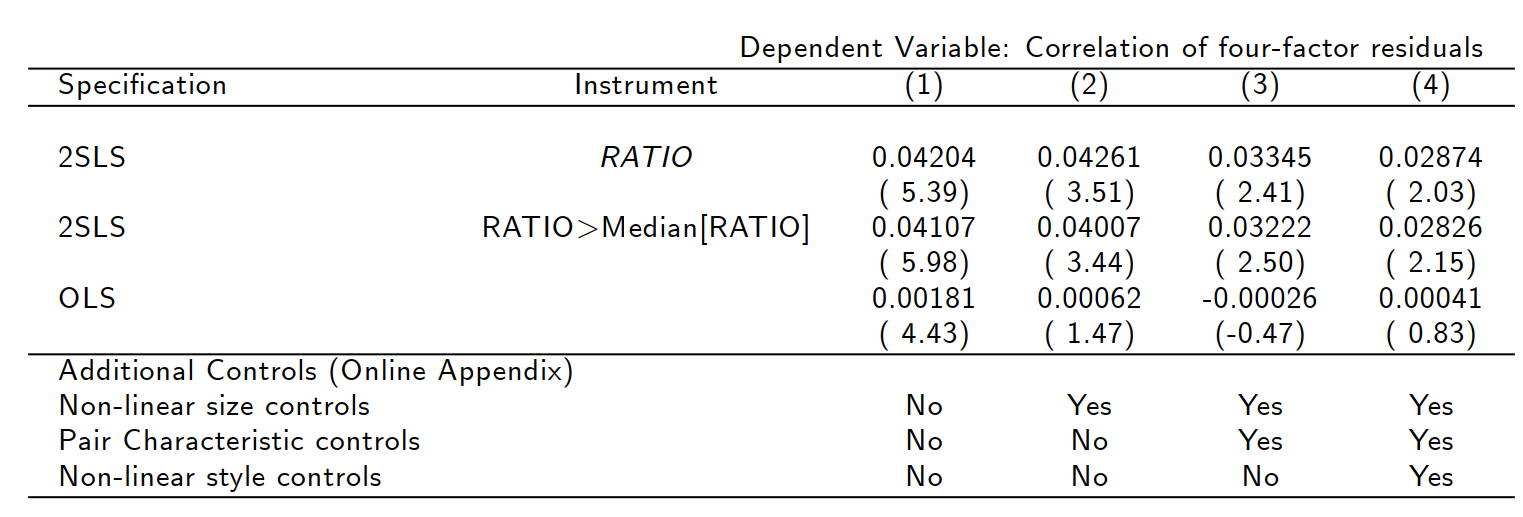
\includegraphics[width=0.7\linewidth]{NSlide.png}
	%\end{figure}
	%\end{frame}
	%
	%
	%\begin{frame}{Connected Stocks}
	%\begin{itemize}
	%\item PFLOAT = The total float capitalizstion of the two stocks in the pair
	%\item PFLOW = The absolute value
	%of the total net flow into the common funds
	%\end{itemize}
	%
	%
	%
	%\begin{figure}[htbp]
	%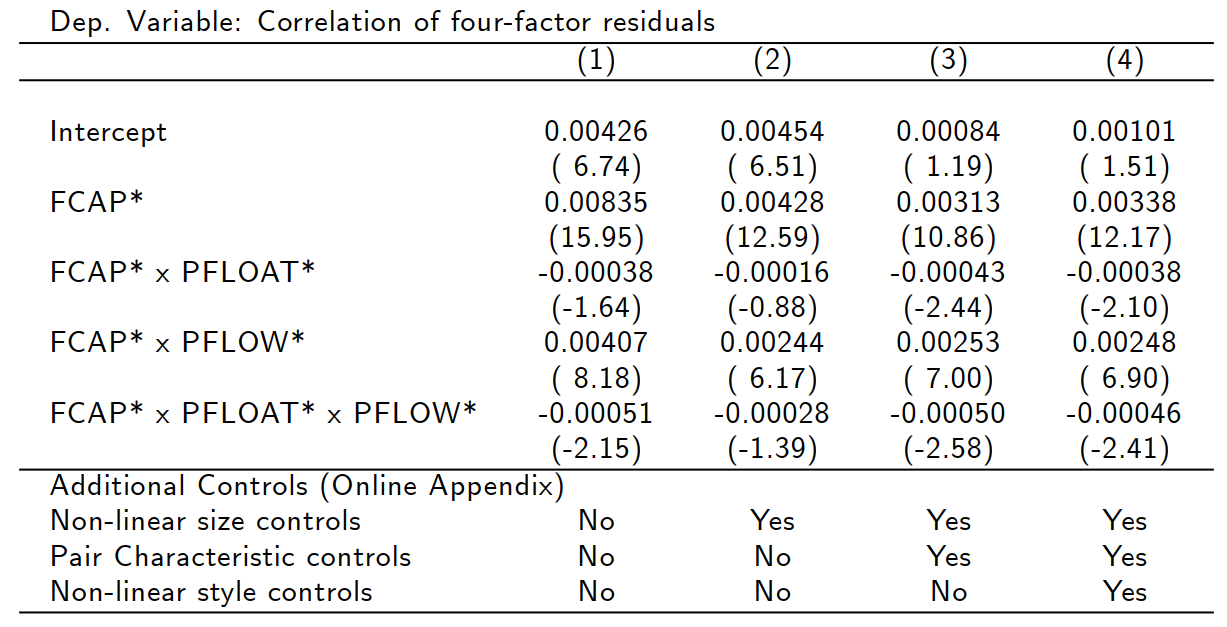
\includegraphics[width=0.65\linewidth]{N2Slide.png}
	%\end{figure}
	%\begin{itemize}
	%\item Prices are more subject to non-fundamental comovement when pressure
	%from net mutual fund trading is high and especially so when the stocks in
	%question have low float and are thus less liquid
	%\end{itemize}
	%\end{frame}
	%
	%
	%
	%\begin{frame}{Connected Stocks}
	%\begin{itemize}
	%\item[]Buy (sell) stocks that have gone down (up) if their connected stocks have gone
	%down (up) as well. The connected return is a confirming signal that the own
	%return will revert
	%\end{itemize}
	%
	%
	%
	%\begin{figure}[htbp]
	%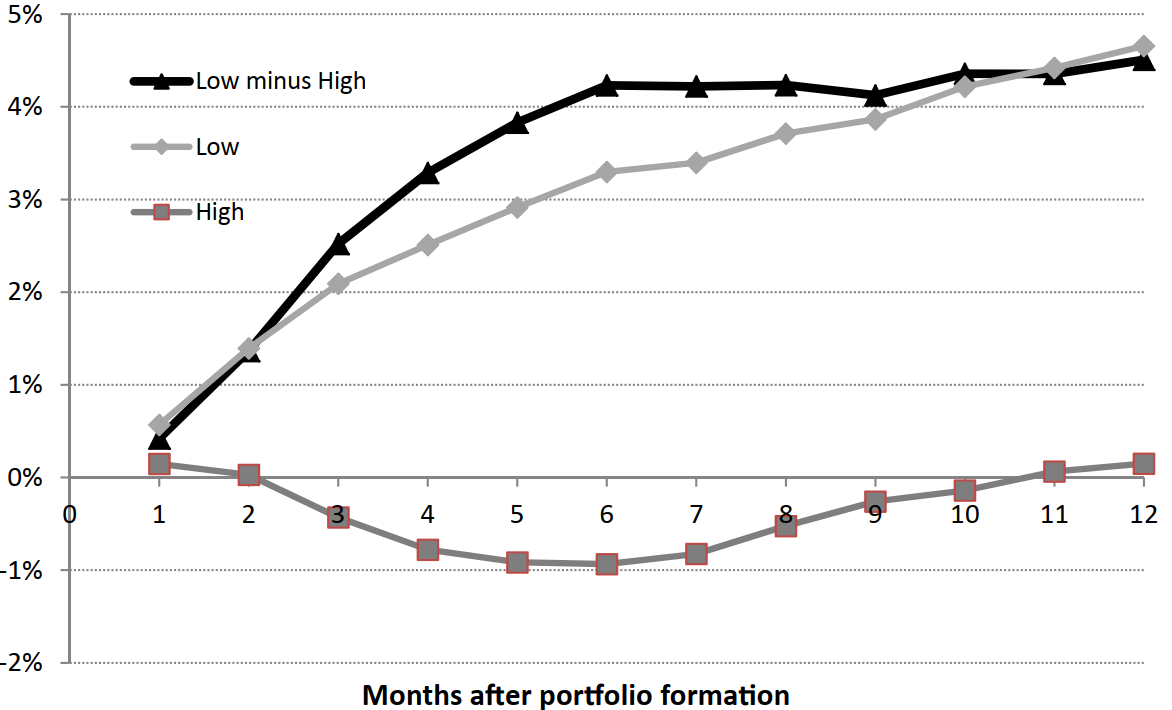
\includegraphics[width=0.5\linewidth]{N3Slide.png}
	%\end{figure}
	%\begin{itemize}
	%\item  low (high) own-return and low (high) connected-return
	%portfolio $ \rightarrow $ low (high) portfolio
	%\end{itemize}
	%\end{frame}
	
	
		\subsection{Main Effect}
	\begin{frame}{Main effect}\label{Grapgh}
		\resizebox{\textwidth}{!}{
	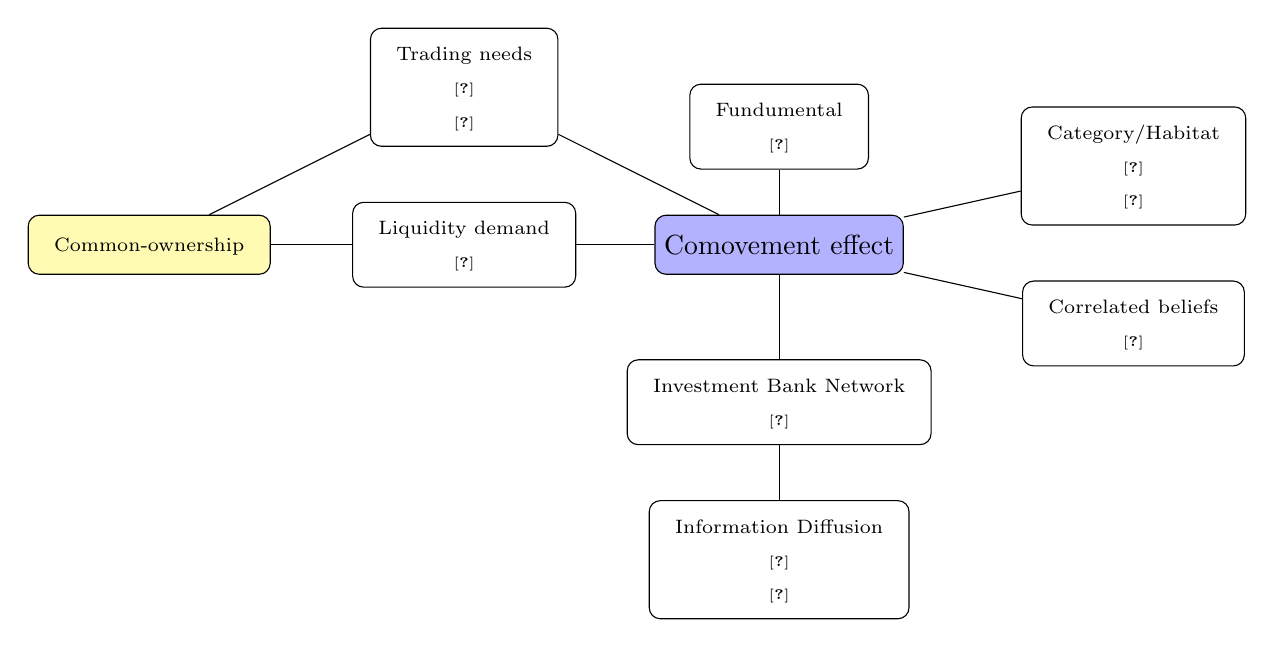
\begin{tikzpicture}[node distance=1cm][every text node part/.style={align=center}]
		
		
		
		\node (comovement) [startstop1] {Comovement effect};
		
		\pause
		
				\node (Fundumental) [startstop3,above of = comovement , yshift=0.5cm , xshift=0cm ] { \begin{tabular}{c}
				\scriptsize	Fundumental	\\ \tiny\cite{shiller1989comovements}
		\end{tabular} };
		
		
		\draw (Fundumental) -> (comovement);
		
		
		\pause
		
		\node (categoryhabitat) [startstop3,above of = comovement , yshift=0cm , xshift=4.5cm ] { \begin{tabular}{c}
				\scriptsize	Category/Habitat	\\ \tiny\cite{barberis2005comovement}\\ \tiny\cite{barberis2003style}
		\end{tabular} };
		
		
		\draw (categoryhabitat) -> (comovement);
		
		\pause
		\node (belief) [startstop3,below of = comovement , yshift=0cm , xshift=4.5cm ] {\begin{tabular}{c}\scriptsize
				Correlated beliefs	\\
				\tiny\cite{david2016correlated}
		\end{tabular}};
		
		\draw (belief) -> (comovement);
		
		\pause
		
		\node (investmentbanking) [startstop3,below of = comovement , yshift=-1cm , xshift=0cm ] {\begin{tabular}{c}\scriptsize
				Investment Bank Network \\
				\tiny\cite{grullon2014comovement}
		\end{tabular}};
		
		\draw (investmentbanking) -> (comovement);
		
		
		
		\pause
		\node (information) [startstop3,below of = investmentbanking , yshift=-1cm , xshift=0cm ] {\begin{tabular}{c}\scriptsize
				Information Diffusion	\\\tiny\cite{pantzalis2017shareholder}\\
				\tiny\cite{HAMEED2019103}
		\end{tabular}};
		
		\draw (information) -> (investmentbanking);
		
		\pause
		
		
		
		
		
		
		
		%% common ownership
		\node (commonownership) [startstop2,left of = comovement , yshift=0cm , xshift=-7cm ] {\begin{tabular}{c}\scriptsize Common-ownership  \end{tabular}};
		\pause
		\node (trading) [startstop3,right of = comovement , yshift=2cm , xshift=-5cm ] { \begin{tabular}{c}
				\scriptsize	Trading needs\\ \tiny \cite{greenwood2011stock} \\  \tiny \cite{AntonPolk}
		\end{tabular} };
		
		\draw (commonownership) -> (trading);
		\draw (trading) -> (comovement);
		\pause
		\node (liquidity) [startstop3,below of = trading , yshift=-1cm , xshift=0cm] {\begin{tabular}{c} \scriptsize Liquidity demand \\ \tiny \cite{Liquidity2016}  \end{tabular}};
		
		\draw (commonownership) -> (liquidity);
		\draw (liquidity) -> (comovement);
		

		
		
%		\node (corporate) [startstop3,below of = liquidity , yshift=-1cm , xshift=0cm ] {  \begin{tabular}{c}
%				\scriptsize	Poor corporate governance	\\ \tiny \cite{khanna2009synchronicity}
%		\end{tabular}};
%		
%		\draw (commonownership) -> (corporate);
%		\draw (corporate) -> (comovement);
	\end{tikzpicture}
}
		
%		\hfill
%		\hyperlink{maineffect}{\beamerbutton{Papers}}
	\end{frame}
	
	\begin{frame}{Our work}
		\begin{itemize}
			\item 
			We use daily records of block-holder ownership for firms
			\item We are not restricted to mutual funds ownership
			\item Furthermore, 80\% of market belongs to the business groups
			\begin{itemize}
				\item Would business groups be able to raise the co-movement of stock returns?
				\begin{itemize}
					\tiny
					\item \cite{cho2015stock}: \\
					The strong co-movement between group returns and
					firm returns is explained by correlated fundamentals. 
					\item \cite{kim2015stock}:\\
					The increase in correlation appears to be driven
					more by non-fundamental factors such as correlated trading, rather
					than fundamental factors such as related-party transactions
				\end{itemize}
			\item Common ownership or business group (indirect common ownership) ?
			\item  Through which channel?
			\end{itemize}
			
		\end{itemize}
	\end{frame}
	
	\normalsize

	
	
	\section{Empirical Studies}
		\subsection{Pair composition}
		\begin{frame}{Pair composition}
			\begin{itemize}
				\item Firms with at least one common owner\\
				\bigskip
								\begin{figure}[htbp]
					\centering
					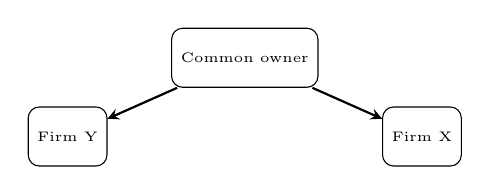
\begin{tikzpicture}[node distance=1cm]
						
						\node (Firm) [startstop3] {\tiny Firm X};
						\node (Firm2) [startstop3,right of = Firm  , xshift=-5.5cm ] {\tiny Firm Y};
						\node (Owner) [startstop3,right of = Firm , yshift=1cm , xshift=-3.25cm ] {\tiny Common owner };
						
						
						\draw[arrow] (Owner) -- node[sloped, anchor=center, above] {} (Firm) ;
						
						\draw[arrow] (Owner) -- node[sloped, anchor=center, above] {} (Firm2) ;
					\end{tikzpicture}
				\end{figure}
			\bigskip
			\pause
				\item In a business group, how can one pair be defined?
				\begin{itemize}
					\item What is the business group?
				\end{itemize}
			\end{itemize}
		\end{frame}
		
		\begin{frame}{Pair Composition and Business Group}{Business Group }
			
			
			\resizebox{0.7\textwidth}{!}{
				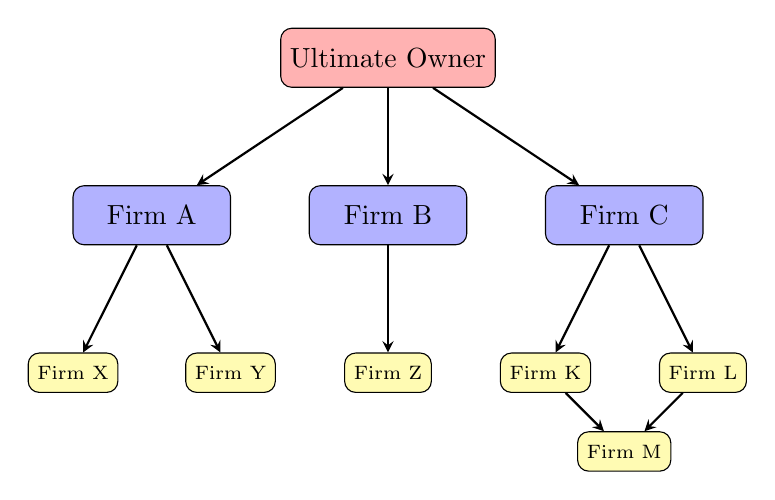
\begin{tikzpicture}[node distance=2cm]
					
					
					\node (UO) [startstop] { $ \text{Ultimate Owner} $};
					\pause
					\node (FirmA) [startstop1,below of = UO,xshift=-3cm] {$ \text{Firm A} $};
					\node (FirmB) [startstop1,right of = FirmA,xshift=1cm] {$ \text{Firm B} $};
					\node (FirmC) [startstop1,right of = FirmB,xshift=1cm] {$ \text{Firm C} $};
					\draw [arrow] (UO) --(FirmA);
					\draw [arrow] (UO) --(FirmB);
					\draw [arrow] (UO) --(FirmC);
					
					\pause
					
					\node (FirmX) [startstop20,below of = FirmA,xshift=-1cm] {$ \scriptsize\text{Firm X} $};
					
					\node (FirmY) [startstop20,below of = FirmA,xshift=1cm] {$ \scriptsize\text{Firm Y} $};
					
					\node (FirmZ) [startstop20,below of = FirmB] {$ \scriptsize\text{Firm Z} $};
					
					\node (FirmK) [startstop20,below of = FirmC , xshift = -1cm] {$ \scriptsize\text{Firm K} $};
					\node (FirmL) [startstop20,below of = FirmC , xshift = 1cm] {$ \scriptsize\text{Firm L} $};
					\node (FirmM) [startstop20,below of = FirmC , yshift = -1 cm] {$ \scriptsize\text{Firm M} $};
					
					
					\draw [arrow] (FirmA) --(FirmX);
					\draw [arrow] (FirmA) --(FirmY);
					
					\draw [arrow] (FirmB) --(FirmZ);
					
					\draw [arrow] (FirmC) --(FirmK);
					\draw [arrow] (FirmC) --(FirmL);
					
					\draw [arrow] (FirmK) --(FirmM);
					\draw [arrow] (FirmL) --(FirmM);
					
					
				\end{tikzpicture}
			}
			
		\end{frame}
		
		
		\begin{frame}{Pair Composition and Business Group}{Pair in the Business Group }
			\begin{columns}
				\column{.5\textwidth}     
				\centering
				{}\\
				\resizebox{\textwidth}{!}{
					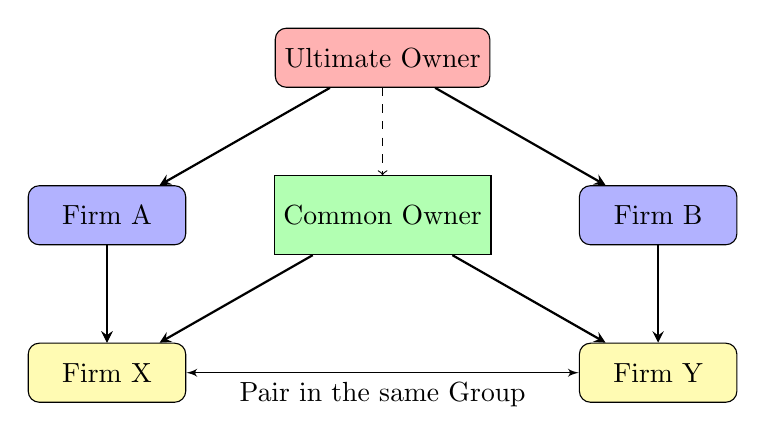
\begin{tikzpicture}[node distance=2cm]
						
						
						\node (start) [startstop] {Ultimate Owner};
						
						
						
						\node (end) [startstop1,below of = start , yshift=0cm , xshift=-3.5cm ] {$ \text{Firm A} $};
						\node (end2) [startstop1,below of = start , yshift=0cm , xshift=3.5cm ] {$ \text{Firm B} $};
						
						
						
						\node (sur) [startstop2 ,below of = end ,yshift=0cm,xshift=0cm] {$ \text{Firm X} $};
						
						
						\node (sur2) [startstop2 ,below of = end2 ,yshift=0cm,xshift=0cm] {$ \text{Firm Y} $};
						
						
						\node (CH) [process, below of = start ,xshift=0] {Common Owner};
						
						
						\draw [arrow] (start) --(end);
						\draw [arrow] (end) --(sur);
						
						\draw [arrow] (start) --(end2);
						
						\draw [arrow] (end) --(sur);
						\draw [arrow] (end2) -- (sur2);
						
						
						\draw [arrow] (CH) -- (sur);
						\draw [arrow] (CH) -- (sur2);
						\draw [dashed ,->] (start) --(CH);
						
						\draw [latex'-latex'] (sur) to [bend right =0]  node[sloped, anchor=center, below] { Pair in the same Group} (sur2);
						
						
					\end{tikzpicture}
				}
				
				\pause
				\column{.5\textwidth}
				\centering  
				{}\\
				\resizebox{\textwidth}{!}{
					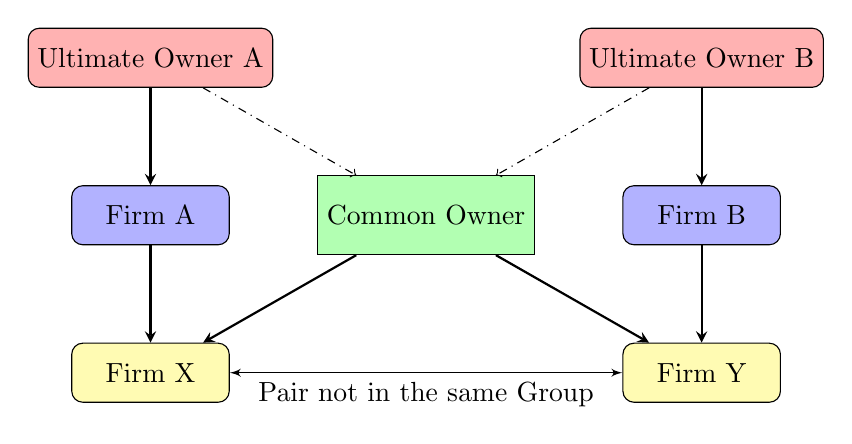
\begin{tikzpicture}[node distance=2cm]
						
						
						\node (start) [startstop] { $ \text{Ultimate Owner A} $};
						\node (start2) [startstop,right of = start,xshift=5cm] {$ \text{Ultimate Owner B} $};
						
						
						\node (CH) [process, below of = start2,xshift=-3.5cm] {Common Owner};
						
						\node (end) [startstop1,below of = start ] {$ \text{Firm A} $};
						
						\node (end2) [startstop1,below of = start2 ,yshift=0cm,xshift=0cm] {$ \text{Firm B} $};
						
						\node (sur) [startstop2 ,below of = end ,yshift=0cm,xshift=0cm] {$ \text{Firm X} $};
						
						\node (sur2) [startstop2,below of = end2 ,yshift=0cm,xshift=0cm] {$ \text{Firm Y} $};
						
						
						
						\draw [arrow] (start) --(end);
						\draw [arrow] (start2) -- (end2);
						
						\draw [arrow] (end) --(sur);
						\draw [arrow] (end2) -- (sur2);
						
						\draw [dash dot,->] (start) -- (CH);
						\draw [dash dot,->] (start2) -- (CH);
						
						\draw [arrow] (CH) -- (sur);
						\draw [arrow] (CH) -- (sur2);
						
						\draw [latex'-latex'] (sur) to [bend right =0]  node[sloped, anchor=center, below] { Pair not in the same Group} (sur2);
						
						
					\end{tikzpicture}
				} 
				
				\end{columns}
		\end{frame}
		
		
		
		
	%	\begin{frame}{Pair Composition and Business Group}{Pair not in any of Business Groups }
	%		\begin{columns}
	%			\column{.5\textwidth}     
	%			\centering
	%			{}\\
	%			
	%			\resizebox{\textwidth}{!}{
	%				\begin{tikzpicture}[node distance=2cm]
	%					
	%					
	%					
	%					\node (CH) [process,yshift = -2cm ,xshift=3.5cm] {Common Owner};
	%					
	%					\node (end) [startstop1,left of = CH ,xshift=-1.5cm ] {$ \text{Firm A} $};
	%					
	%					\node (end2) [startstop1,right of = CH ,yshift=0cm,xshift=1.5cm] {$ \text{Firm B} $};
	%					
	%					\node (sur) [startstop2 ,below of = end ,yshift=0cm,xshift=0cm] {$ \text{Firm X} $};
	%					
	%					\node (sur2) [startstop2,below of = end2 ,yshift=0cm,xshift=0cm] {$ \text{Firm Y} $};
	%					
	%					
	%					\draw [arrow] (end) --(sur);
	%					\draw [arrow] (end2) -- (sur2);
	%					
	%					
	%					\draw [arrow] (CH) -- (sur);
	%					\draw [arrow] (CH) -- (sur2);
	%					
	%					\draw [latex'-latex'] (sur) to [bend right =0]  node[sloped, anchor=center, below] { Pair not in Groups} (sur2);
	%					
	%					
	%				\end{tikzpicture}
	%			} 
	%			
	%			\column{.5\textwidth}
	%			\centering  
	%			{}\\
	%			
	%			\resizebox{\textwidth}{!}{
	%				\begin{tikzpicture}[node distance=2cm]
	%					
	%					
	%					\node (start) [startstop] { $ \text{Ultimate Owner} $};
	%					
	%					
	%					\node (CH) [process, below of = start,xshift=3.5cm] {Common Owner};
	%					
	%					\node (end) [startstop1,below of = start ] {$ \text{Firm A} $};
	%					
	%					\node (end2) [startstop1,right of = CH ,yshift=0cm,xshift=1.5cm] {$ \text{Firm B} $};
	%					
	%					\node (sur) [startstop2 ,below of = end ,yshift=0cm,xshift=0cm] {$ \text{Firm X} $};
	%					
	%					\node (sur2) [startstop2,below of = end2 ,yshift=0cm,xshift=0cm] {$ \text{Firm Y} $};
	%					
	%					
	%					
	%					\draw [arrow] (start) --(end);
	%					
	%					\draw [arrow] (end) --(sur);
	%					\draw [arrow] (end2) -- (sur2);
	%					
	%					\draw [dash dot,->] (start) -- (CH);
	%					
	%					\draw [arrow] (CH) -- (sur);
	%					\draw [arrow] (CH) -- (sur2);
	%					
	%					\draw [latex'-latex'] (sur) to [bend right =0]  node[sloped, anchor=center, below] { Pair not in Groups} (sur2);
	%					
	%					
	%				\end{tikzpicture}
	%			} 
	%			
	%		\end{columns}
	%	\end{frame}
		
		
		
			\begin{frame}{Data Summary}
			\begin{itemize}
				\item We use blockholders' data from 2014/03/25 \scriptsize{(1393/01/06)} \normalsize to 2020/03/18 \scriptsize (1398/12/28)  \normalsize
				\begin{itemize}
					\item Includes of 72 Months
					\item Consists of 618 firm inculding 562 firm with common owners
					
				\end{itemize}
			\end{itemize}
			
			\begin{table}[htbp]
				\centering
				\resizebox{0.8\textwidth}{!}
				{
					\begin{tabular}{lrrrrrr}
\toprule
Year &  2014 &  2015 &  2016 &  2017 &  2018 &  2019 \\
\midrule
No. of Firms                        &   365 &   376 &   446 &   552 &   587 &   618 \\
No. of Blockholders                 &  1606 &  1676 &  2099 &  2978 &  3374 &  3416 \\
No. of Groups                       &    38 &    41 &    43 &    44 &    40 &    43 \\
No. of Firms in Groups              &   249 &   268 &   300 &   336 &   346 &   375 \\
Ave. Number of group Members        &     7 &     7 &     7 &     8 &     9 &     9 \\
Ave. ownership of each Blockholders &    18 &    19 &    18 &    17 &    18 &    19 \\
Med. ownership of each Blockholders &     5 &     4 &     4 &     4 &     4 &     4 \\
Ave. Number of Owners               &     7 &     6 &     6 &     7 &     7 &     7 \\
Ave. Block. Ownership               &    77 &    77 &    75 &    76 &    75 &    72 \\
\bottomrule
\end{tabular}

				}
			\end{table}
			
		\end{frame}
		
		
		
		\begin{frame}{Pair Composition}
			\begin{itemize}
			
				\item Pairs consist of two firms  with at least one common owner
				\begin{itemize}
					\item  93442 unique pairs which is 25\% of possible pairs 
					\tiny ($ \frac{612*611}{2}= 373932 $)
					\normalsize
				\end{itemize}
			\end{itemize}
			
			\begin{table}[htbp]
				\centering
				{
					\footnotesize
				\begin{tabular}{lrrrr}
\toprule
{} &  mean &   min &  Median &   max \\
\midrule
Number of unique paris &  5000 &  3370 &    5097 &  6366 \\
\bottomrule
\end{tabular}

					
				}
			\end{table}
			
			
			\begin{table}
				\resizebox{0.7\textwidth}{!}
				{
					\begin{tabular}{lrrrrrr}
\toprule
year &   1393 &   1394 &   1395 &   1396 &   1397 &   1398 \\
\midrule
No. of Pairs                          &  20876 &  21187 &  27784 &  41449 &  47234 &  67232 \\
No. of Groups                         &     37 &     40 &     42 &     43 &     39 &     43 \\
No. of Pairs not in Groups            &  11452 &  11192 &  15351 &  26530 &  29182 &  43433 \\
Number of Pairs not in the same Group &   7962 &   8731 &  10971 &  12916 &  15366 &  20745 \\
Number of Pairs in the same Group     &    923 &    955 &   1099 &   1260 &   1536 &   1774 \\
Average Number of Common owner        &      1 &      1 &      1 &      1 &      1 &      1 \\
Med. Number of Common owner           &      1 &      1 &      1 &      1 &      1 &      1 \\
Average Percent of each blockholder   &     19 &     19 &     19 &     19 &     19 &     20 \\
Med. Percent of each blockholder      &     13 &     12 &     12 &     12 &     12 &     14 \\
Average Number of Pairs in one Group  &     31 &     30 &     30 &     34 &     39 &     44 \\
Med. Number of Pairs in one Group     &      8 &     10 &      8 &     10 &      9 &     10 \\
Average Number of Owners              &      5 &      5 &      5 &      5 &      4 &      5 \\
Med. Number of Owners                 &      5 &      5 &      5 &      5 &      4 &      5 \\
Average Block. Ownership              &     73 &     73 &     72 &     70 &     70 &     70 \\
Med. Block. Ownership                 &     73 &     73 &     73 &     71 &     71 &     71 \\
\bottomrule
\end{tabular}

				}
			\end{table}% 
			
		\end{frame}  
		
		
		
	
	%	\begin{frame}{Number of Pairs}
	%		\begin{figure}[htbp]
	%			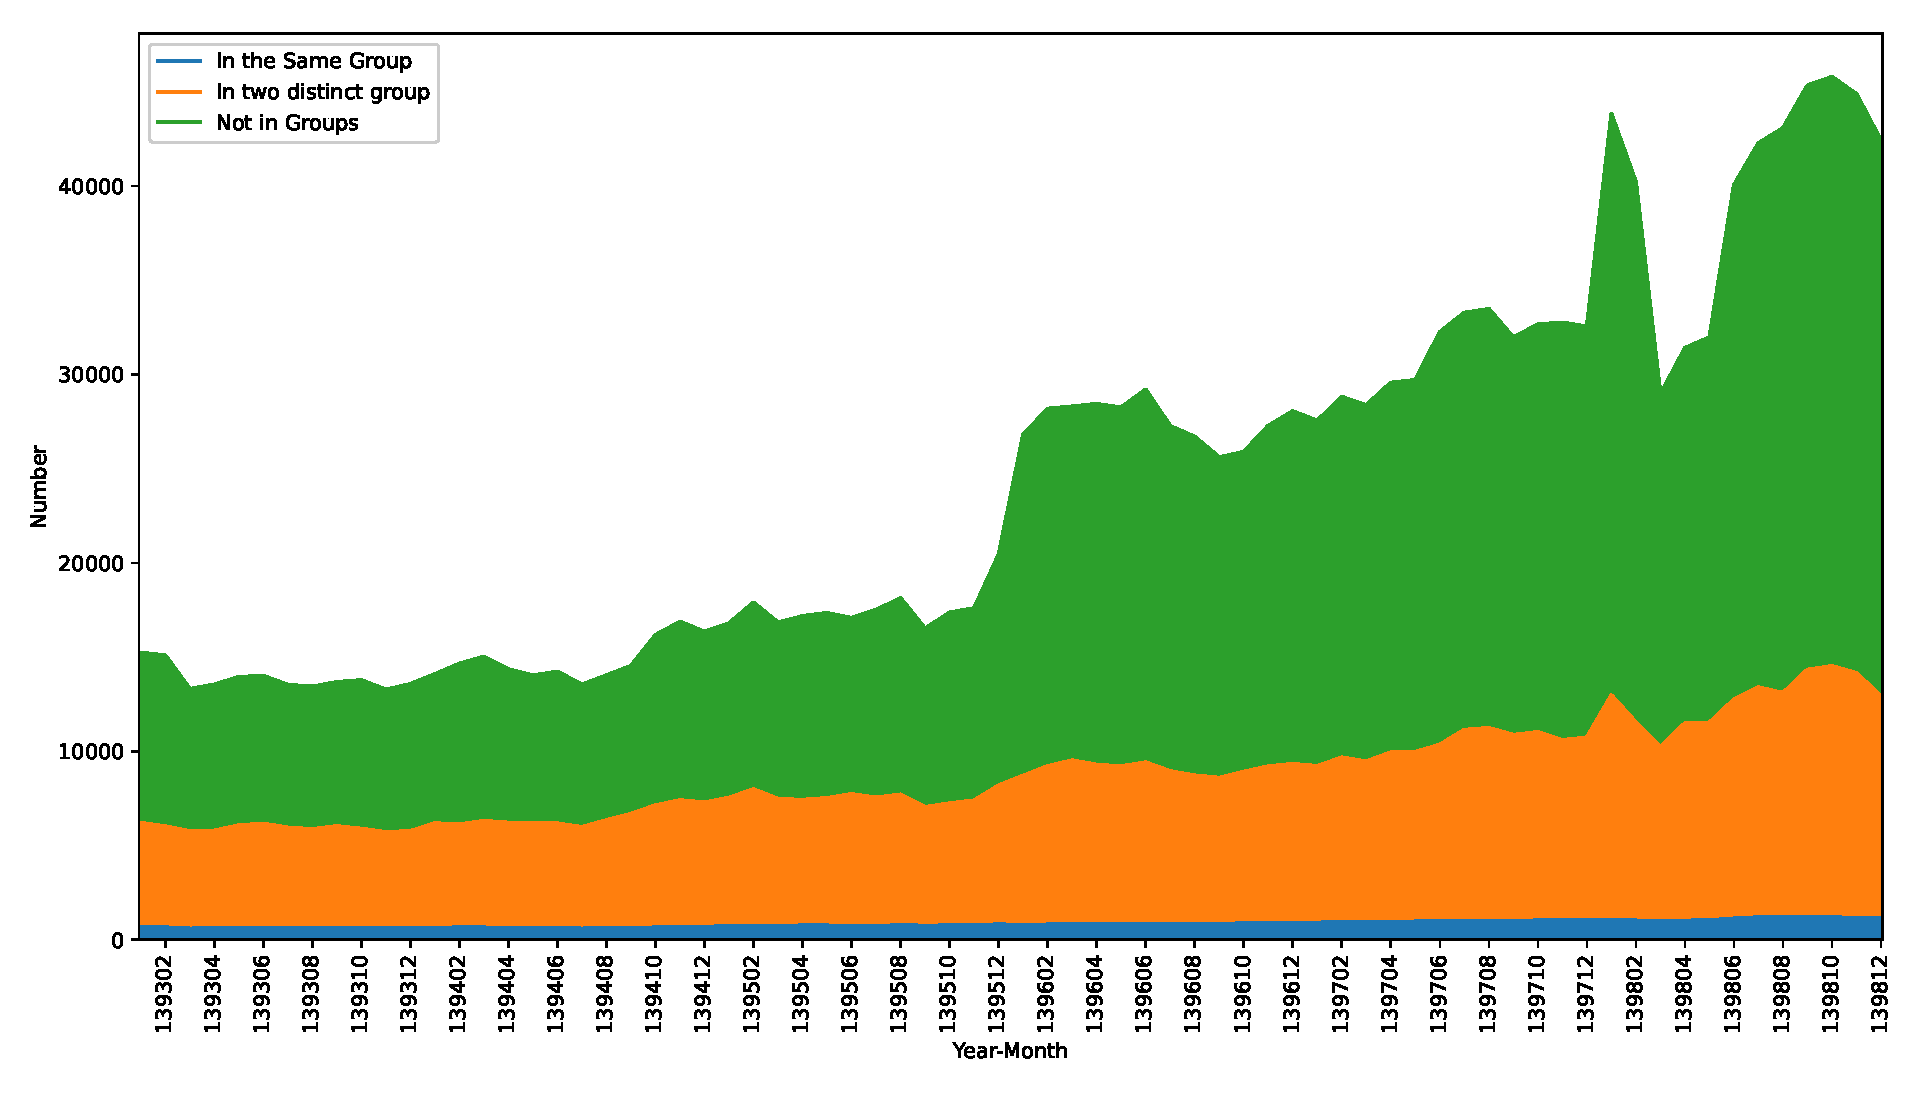
\includegraphics[width=0.9\linewidth]{Output/idMonth.eps}
	%		\end{figure}
	%	\end{frame}
	%	
		
		
		
		
	%	\begin{frame}{FCA's time series}
	%		\begin{figure}
	%			\centering  
	%			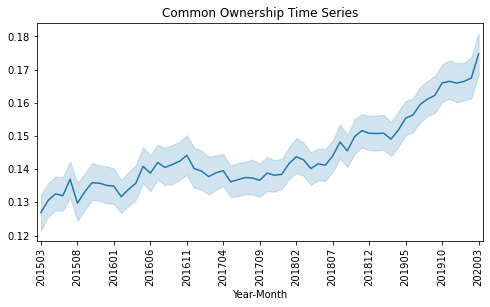
\includegraphics[width=0.9\linewidth]{"Output/FCAtimeSeries.eps"}
	%			
	%		\end{figure} 
	%	\end{frame}
	%
	%	\begin{frame}{FCA's time series}
	%		\begin{columns}
	%			\column{.5\textwidth}  
	%			\begin{figure}
	%				\centering  
	%				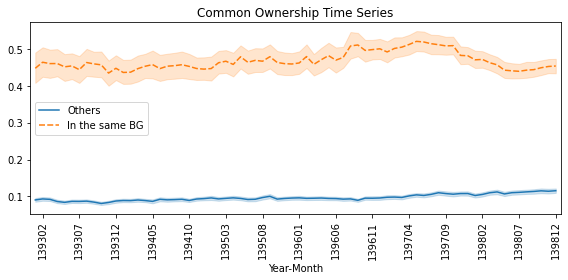
\includegraphics[width=\linewidth]{"Output/FCAtimeSeriesBG.eps"}
	%				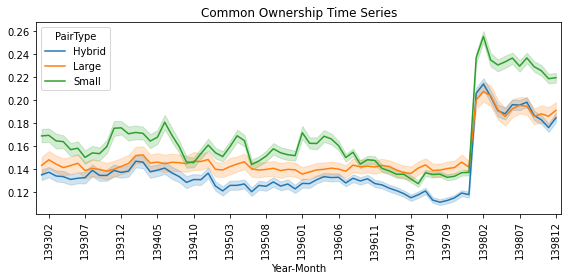
\includegraphics[width=\linewidth]{"Output/FCAtimeSeriesPairType.eps"}
	%			\end{figure}    
	%			\column{.5\textwidth}
	%			\begin{figure}
	%				\centering  
	%				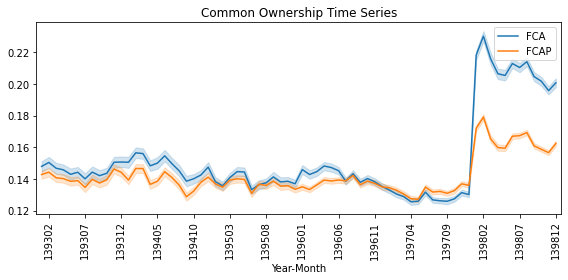
\includegraphics[width=\linewidth]{"Output/FCAComparetimeSeries.eps"}
	%			\end{figure}
	%          
	%		\end{columns}
	%
	%\end{frame}
	%
	%	\begin{frame}{Group affiliated firm's time series}
	%		\begin{columns}
	%	\column{.5\textwidth}  
	%	\begin{figure}
	%	\centering  
	%	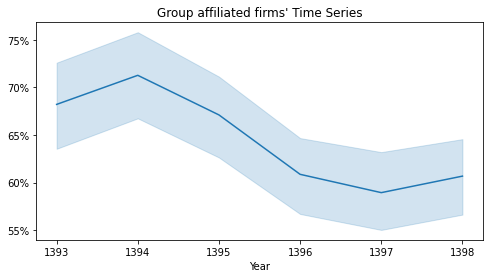
\includegraphics[width=\linewidth]{"Output/BGtimeSeries.eps"}
	%	
	%\end{figure}  
	%	\column{.5\textwidth}
	%	\begin{figure}
	%	\centering  
	%	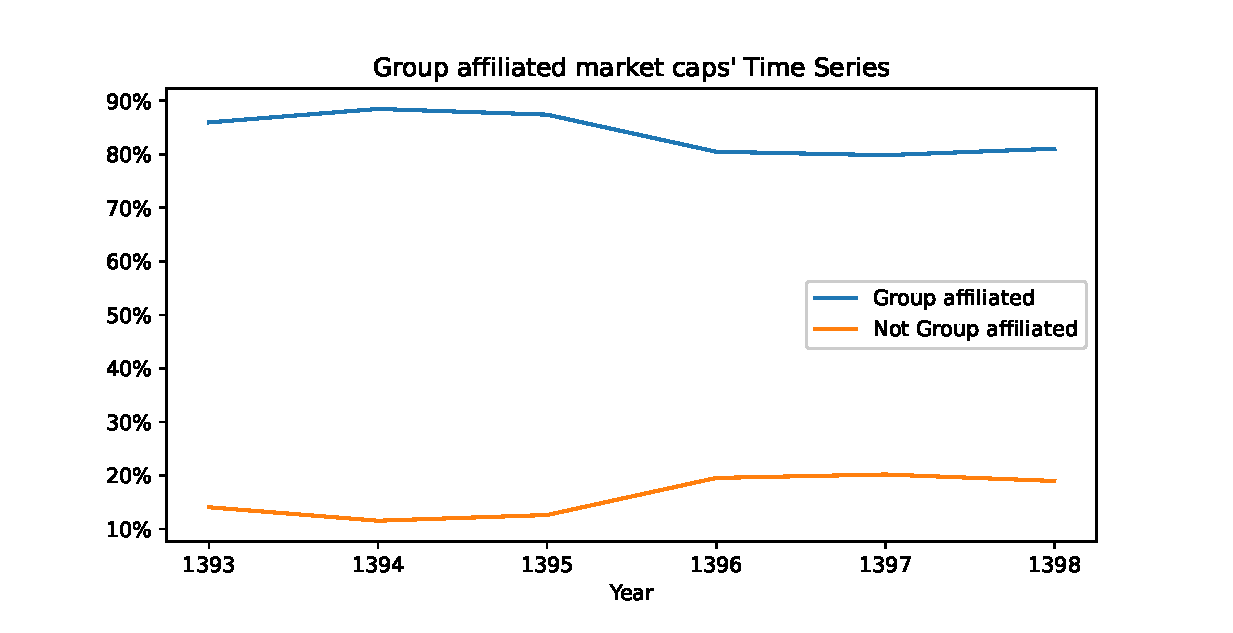
\includegraphics[width=\linewidth]{"Output/BGMarketCaptimeSeries.eps"}
	%	
	%\end{figure} 
	%	
	%\end{columns}
	%\end{frame}
	
	
	
	
		
	
	\subsection{Measuring Common-ownership}
	\begin{frame}{Common-ownership measurements}\label{mainmeasure}
			\begin{columns}[t]
				\column{0.5\textwidth}  
				\centering
				Model based measures
				\\
				
				\begin{itemize}
					\item \color{blue} \scriptsize $
					\text{HJL}_I^A(A,B) = \sum_{i\in I^{A,B}}\frac{\alpha_{i,B}}{\alpha_{i,A} + \alpha_{i,B}}     $  
					\normalcolor
					\tiny 
					
					\cite{harford2011institutional}
					
					
					\item \color{blue} \scriptsize$   \text{MHHI} = \sum_{j} \sum_k s_j s_k \frac{\sum_i \mu_{ij} \nu_{ik}}{\sum_i \mu_{ij} \nu_{ij}}   $ \tiny   \normalcolor
					
					\cite{azar2018anticompetitive}
					
					\item \color{blue} \scriptsize $   \text{Top5}_j = \frac{1}{n-1}\sum_i^5 \sum_{j\neq k} \nu_{ik}   $ \tiny \normalcolor 
					
					\cite{anton2020common} 
					
					\item \color{blue} \scriptsize $   \kappa_{ij} = \cos(\nu_i,\nu_j) . \sqrt{\frac{IHHI_j}{IHHI_i}}   $ \tiny \normalcolor 
					
					\cite{backus2020theory}
					
					\item \color{blue} \scriptsize$   \text{GGL}^A(A,B) = \sum_{i = 1}^{I} \alpha_{i,A}g(\beta_{i,A})\alpha_{i,B}   $ \tiny \normalcolor 
					
					\cite{gilje2020s} , \cite{Lewellen2021}
					
					
					\item \color{blue} \scriptsize $   \text{MHHI}_\text{Delta}= \sum_{j = 1}^{J} \sum_{k\neq j}^{K} \frac{\sum_{i = 1}^{N} w_j * w_k * \mu_{i,j} * \mu_{i,k}}{\sum_{i = 1}^{N}  \mu_{i,j} * \mu_{i,k} }  $ \tiny \normalcolor 
					
					\cite{LEWELLEN2021b}
					\normalsize
					
					
					
				\end{itemize}
				
				
				\pause
				\column{0.5\textwidth}
				\centering
				Ad-hoc measures
				\begin{itemize}
					\item \scriptsize \color{orange}  $   \text{Overlap}_{AP}(A,B)= \sum_{i\in I^{A,B}} \alpha_{i,A}\frac{\bar{\nu}_A}{\bar{\nu}_A +\bar{\nu}_B } + \alpha_{i,B}\frac{\bar{\nu}_B}{\bar{\nu}_A +\bar{\nu}_B } $  \normalcolor\\
					\tiny\cite{AntonPolk} \\ 
					
					\item \scriptsize\color{orange}  $   \text{Overlap}_{Count}{{(A,B)}}= \sum_{i\in I^{A,B}} 1 $  \normalcolor\\
					\tiny \cite{he2017product},\cite{he2019internalizing} \\ 
					
					
					\item \scriptsize\color{orange}  $   \text{Overlap}_{Min}(A,B)= \sum_{i\in I^{A,B}} min\{\alpha_{i,A},\alpha_{i,B}\} $  \normalcolor\\
					\tiny \cite{newham2018common}  \\ 
					
					
					
					
					
					\item \scriptsize\color{orange}  $   \text{Overlap}_{HL}(A,B)= \sum_{i\in I^{A,B}} \alpha_{i,A} \times \sum_{i\in I^{A,B}} \alpha_{i,B} $  \normalcolor\\
					
					\tiny \cite{hansen1996externalities} , \cite{freeman2019effects} \\ 
					
				\end{itemize}
				
			\end{columns}
			\pause
			\begin{block}{\scriptsize Selected measure }
				\scriptsize
				We need a pair-level measure, which is bi-directional, so we use the AP measure. 
			\end{block}
			\hfill
			\hyperlink{measuredetail}{\beamerbutton{Measues' detail}}
		\end{frame}

	\begin{frame}{Measuring Common-ownership}\label{Intuition}
				\begin{columns}
			\column{.5\textwidth}    
			\centering  
						\cite{AntonPolk}
								\begin{align*}
									\boxed{FCAP_{ij,t} = \frac{\sum_{f = 1}^{F} (S^f_{i,t}P_{i,t}+S^f_{j,t}P_{j,t})}{S_{i,t}P{i,t} + S_{j,t}P{j,t}}}
								\end{align*} 
%			\pause
			\column{.5\textwidth}
			\centering
			SQRT
						\begin{align*}
						\footnotesize	\boxed{    MFCAP_{ij,t} =           [\frac{\sum_{f =1}^{F}(\sqrt{S^f_{i,t}P_{i,t}}+\sqrt{S^f_{j,t}P_{j,t}})}{\sqrt{S_{i,t}P{i,t}} + \sqrt{S_{j,t}P{j,t}}}]^2 }
						\end{align*}     				         
		\end{columns}
	\pause
		\begin{block}{Intuition}
			If for a pair of stocks with n mutual owners, all owners have even shares of each firm's market cap, then the proposed indexes will be equal to n.
			\hyperlink{Proof}{\beamerbutton{Proof}}
		\end{block}
		
	\end{frame}
	
	
				\begin{frame}{MFCAP vs. FCAP Summary}
					\begin{table}[htbp]
						\centering
						\resizebox{\textwidth}{!}
						{
							\begin{tabular}{lrrrrrrrrrr}
\toprule
\multirow{2}{*}{Subset}& \multicolumn{5}{c}{MFCAP} & \multicolumn{5}{c}{FCAP} \\
\cmidrule(lr){2-6} \cmidrule(lr){7-11}
&       mean &    std &    min & median &    max &         mean &    std &    min & median &    max \\
\midrule
All               &  0.15 &  0.24 &  0.00 &   0.06 &  4.62 &  0.12 &  0.16 &  0.0 &   0.05 &  0.97 \\
Same Group        &  0.47 &  0.41 &  0.00 &   0.41 &  4.04 &  0.38 &  0.25 &  0.0 &   0.37 &  0.97 \\
Not Same Group    &  0.10 &  0.16 &  0.00 &   0.04 &  2.90 &  0.08 &  0.11 &  0.0 &   0.04 &  0.97 \\
Same Industry     &  0.34 &  0.41 &  0.01 &   0.18 &  4.04 &  0.25 &  0.24 &  0.0 &   0.16 &  0.96 \\
Not Same Industry &  0.12 &  0.19 &  0.00 &   0.05 &  4.62 &  0.10 &  0.14 &  0.0 &   0.05 &  0.97 \\
\bottomrule
\end{tabular}
  }          
					\end{table}%
					\begin{block}{Results}
						\small
						\begin{itemize}
							\item By the proposed measurement, common ownership increases
							\item Common ownership is greater in pairs that  are in the same business group and insutry
						\end{itemize}
					\end{block}
				\end{frame}
		
			
			\begin{frame}{MFCAP vs. FCAP Distributions}{Monthly}
				\label{Monthly1}
				\begin{columns}
					\column{.33\textwidth}  
					\begin{figure}
						\centering  
						\includegraphics[width=\linewidth]{"MHistFCA.eps"}\\
						\includegraphics[width=\linewidth]{"MHistFCAP.eps"}
					\end{figure}  
				\pause   
					\column{.33\textwidth}
					\begin{figure}
						\centering  
						\includegraphics[width=\linewidth]{"MHistlnFCA.eps"}\\
						\includegraphics[width=\linewidth]{"MHistlnFCAP.eps"}
					\end{figure}
				\pause
					\column{.33\textwidth}
					\begin{figure}   
						\centering
						\includegraphics[width=\linewidth]{"MHistNFCA.eps"}  \\
						\includegraphics[width=\linewidth]{"MHistNFCAP.eps"}   \end{figure}            
				\end{columns}
			\end{frame}
			
			
	
	\subsection{Correlation Calculation}
	\begin{frame}{Correlation Calculation}{4 Factor + Industry}
		
		\begin{enumerate}
			\item Frist Step:\\
			\footnotesize
			Estimate each of these models on periods of three month:
			\begin{itemize}
				\item CAPM + Industry (2 Factor): 
				\begin{equation*}
					\begin{split}
						R_{i,t} =\alpha _{i}&+\beta _{mkt,i}{\mathit {R}}_{M,t} + \beta_{Ind,i}{\mathit {R}}_{Ind,t} + \boxed{\varepsilon_{i,t}}
					\end{split}
					\label{e12}
				\end{equation*}
				\item 4 Factor : 
				\begin{equation*}
					\begin{split}
						R_{i,t} =\alpha _{i}&+\beta _{mkt,i}{\mathit {R}}_{M,t} + \\
						&+\beta _{HML,i}{\mathit {HML}}_{t}+\beta _{SMB,i}{\mathit {SMB}}_{t}+\beta _{UMD,i}{\mathit {UMD}}_{t}+ \boxed{\varepsilon_{i,t}}
					\end{split}
					\label{e11}
				\end{equation*}
				
				\item 4 Factor + Industry (5 Factor) : 
				\begin{equation*}
					\begin{split}
						R_{i,t} =\alpha _{i}&+\beta _{mkt,i}{\mathit {R}}_{M,t} + \beta_{Ind,i}{\mathit {R}}_{Ind,t} \\
						&+\beta _{HML,i}{\mathit {HML}}_{t}+\beta _{SMB,i}{\mathit {SMB}}_{t}+\beta _{UMD,i}{\mathit {UMD}}_{t}+ \boxed{\varepsilon_{i,t}}
					\end{split}
					\label{e10}
				\end{equation*}
			\end{itemize}
			\normalsize
			\item Second Step:\\
			\footnotesize
			Calculate monthly correlation of each stock pair’s daily abnormal returns (residuals)
			
		\end{enumerate}
		
	\end{frame}
	%   
	%   
	%   
	%
	%   
	\begin{frame}{Correlation Calculation Results}
		
		
%		\begin{table}[htbp]
%			\centering 
%			\scriptsize
%			{
%				\begin{tabular}{lcccc}\hline\hline
%					Factors  & \multicolumn{1}{l}{mean} & \multicolumn{1}{l}{std} & \multicolumn{1}{l}{min} & \multicolumn{1}{l}{max} \\
%					\hline
%					SMB     & 0.19  & 1.47  & -5.64 & 19.52 \\
%					HML   & -0.12 & 1.39  & -4.90 & 23.20 \\
%					$ \text{Winner}-\text{Loser} $   & 0.69  & 1.06  & -2.61 & 8.58 \\
%					$ \text{Market} $  & 0.24  & 1.23  & -4.71 & 4.89 \\\hline\hline
%			\end{tabular}                          }
%		\end{table}
%		
		
		
		\begin{table}[htbp]
			\centering 
			\scriptsize
			\resizebox{0.8\textwidth}{!}{
				\begin{tabular}{lrrrrr}
\toprule
{} &   mean &    std &  min &  median &  max \\
\midrule
 CAPM + Industry    &  0.018 &  0.205 & -1.0 &   0.018 &  1.0 \\
4 Factor            &  0.031 &  0.206 & -1.0 &   0.027 &  1.0 \\
4 Factor + Industry &  0.014 &  0.204 & -1.0 &   0.012 &  1.0 \\
\bottomrule
\end{tabular}
              
			}
		\end{table}
		
		
		\begin{block}{Conclusion}
			\scriptsize
			We use the 4 Factor + Industry model to control for exposure to systematic risk because it almost captures all correlations between two firms in each pair.
		\end{block}
	\end{frame}
	
	
	\begin{frame}{Future Correlation via $ FCA $}
		\begin{figure}
			\centering  
			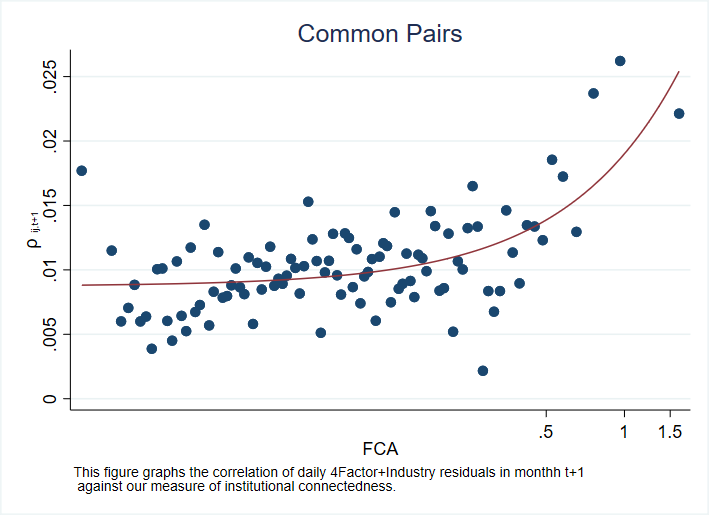
\includegraphics[width=0.85\linewidth]{"Output/mcorr50.eps"}
		\end{figure}
	\end{frame}   
	
	\subsection{Controls}
	\begin{frame}{Controls}
		\begin{itemize}
%			\item $ \rho_{t} $ : Current period correlation
			
			\item \textbf{SameGroup} : Dummy variable for whether the two stocks belong to the same business group.
			
			
			\item \textbf{SameIndustry} : Dummy variable for whether the two stocks belong to the same Industry.
			
			\item \textbf{SameSize} : The negative of absolute difference in percentile ranking of size across a pair
			
			\item \textbf{SameBookToMarket} :The negative of absolute difference in percentile ranking of the book to market ratio across a pair
			
			\item \textbf{CrossOwnership}: The maximum percent of cross-ownership between two firms
		\end{itemize}
	\end{frame}
	
	
	
	\begin{frame}{Industry \& Business group}
				\begin{table}[htbp]
			\centering \scriptsize
			{
				
    \begin{tabular}{lcc}\hline\hline
    {Type of Pairs} & {Yes} &{No} \\
    \hline
    \addlinespace
    {SameIndustry} & 1760  & 16739 \\
          & \tiny(10\%) & \tiny (90\%) \\
          \addlinespace
{SameGroup} & 1118  & 17381 \\
          & \tiny(6\%) & \tiny (94\%) \\
          \addlinespace
{SameGroup \& SameIndustry} & 492  & 18007 \\
          & \tiny(3\%) & \tiny (97\%) \\    
                
          \hline\hline
    \end{tabular}%
			}
		\end{table}
		\begin{figure}[htbp]
			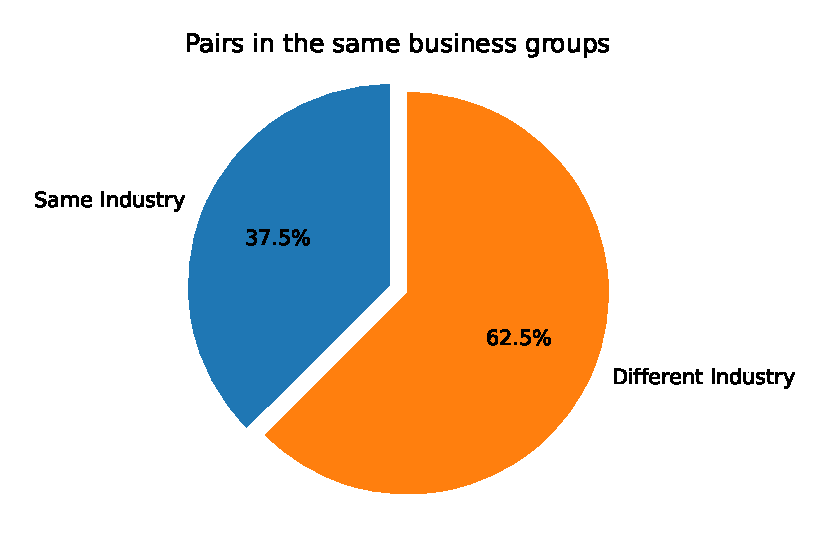
\includegraphics[width=0.45\linewidth]{Output/sameIndustryinBG.eps}
			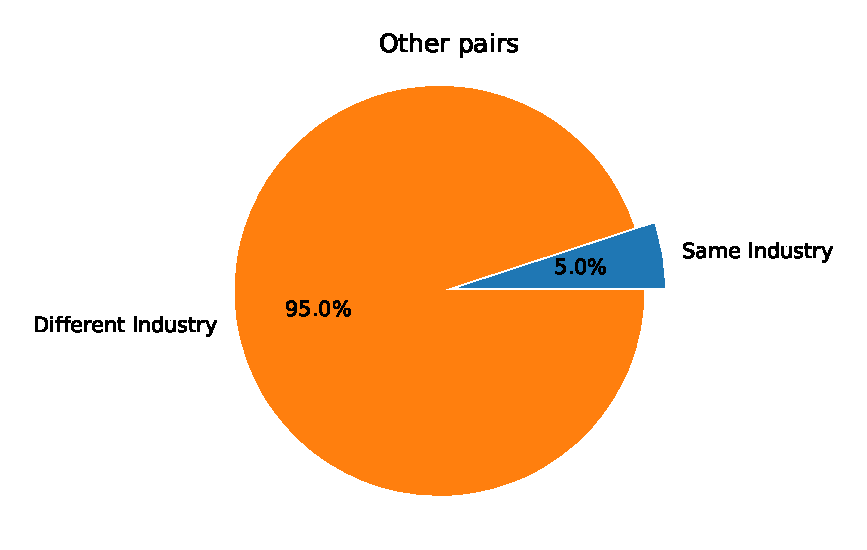
\includegraphics[width=0.45\linewidth]{Output/sameIndustryNoinBG.eps}
			
		\end{figure}
	\end{frame}
	
	\begin{frame}{Business group}{Pairs' characteristic}
		\begin{figure}[htbp]
			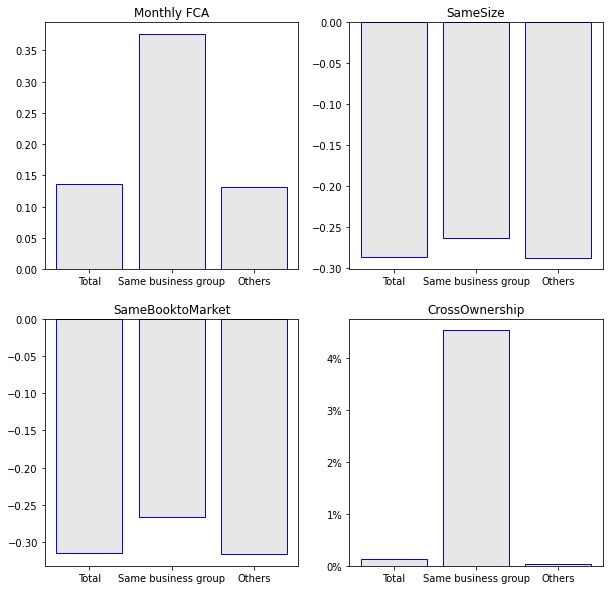
\includegraphics[width=0.6\linewidth]{Output/BGSummary.eps}
			
		\end{figure}
	\end{frame}
	
	
	
	
	\begin{frame}{Summary of Controls}{Variables' distribution } \label{Monthly2}

		
		\begin{table}[htbp]
			\centering 
			\scriptsize
			{
				\begin{tabular}{lrrrrrrr}\hline\hline
          & \multicolumn{1}{l}{mean} & \multicolumn{1}{l}{std} & \multicolumn{1}{l}{min} & 25\%  & 50\%  & 75\%  & \multicolumn{1}{l}{max} \\
          \hline
          
          SameIndustry & 0.10  & 0.29  & 0.00  & 0.00  & 0.00  & 0.00  & 1.00 \\
          SameGroup & 0.06  & 0.23  & 0.00  & 0.00  & 0.00  & 0.00  & 1.00 \\
          Size1 & 0.72  & 0.21  & 0.01  & 0.58  & 0.78  & 0.91  & 1.00 \\
          Size2 & 0.43  & 0.25  & 0.00  & 0.23  & 0.42  & 0.62  & 0.99 \\
          SameSize & -0.29 & 0.21  & -0.97 & -0.42 & -0.24 & -0.12 & 0.00 \\
          BookToMarket1 & 0.53  & 0.26  & 0.00  & 0.34  & 0.54  & 0.73  & 1.00 \\
          BookToMarket2 & 0.52  & 0.24  & 0.00  & 0.34  & 0.52  & 0.71  & 1.00 \\
          SameBookToMarket & -0.30 & 0.19  & -0.99 & -0.42 & -0.26 & -0.15 & 0.00 \\
          MonthlyCrossOwnership & 0.01  & 0.05  & 0.00  & 0.00  & 0.00  & 0.00  & 0.96 \\
          
    
    \hline\hline
            \end{tabular}
			}
		\end{table}
		
		
	\end{frame}
	
	%\begin{frame}{Regression Summary}
	%\begin{itemize}
	%\item \textbf{Controls} :  We use the percentile rank of a particular characteristic for each stock in regression.
	%\item \textbf{Interaction} : We use the interaction between percentile rankings for a particular characteristic across a pair in regression.
	%\end{itemize}
	%\end{frame}
	
	\section{Methodology}
	
	\begin{frame}{Fama-MacBeth Estimation}
		\begin{itemize}
			\item Fama-MacBeth regression analysis is implemented using a two-step procedure. 
			\begin{itemize}
				\item The first step is to
				run periodic cross-sectional regression for dependent variables using data of each period.
				\item[]
				\item
				The second step is to analyze the time series
				of each regression coefficient to determine whether the average coefficient differs from zero.
			\end{itemize}
			
		\end{itemize}
	\end{frame}
	
	\begin{frame}{Fama-MacBeth (1973)}
		\begin{itemize}
			
			\item Two Step Regression
			\begin{itemize}
				\item First Step
				\begin{equation*}
					\begin{array}{c}
						Y_{i1} = \delta_{0,1} + \delta_{1,1}^1 X^1_{i,1} + \dots  + \delta_{k,1}^k X^k_{i,1}  + \varepsilon_{i,1}\\
						\vdots\\
						Y_{iT} = \delta_{0,1} + \delta_{1,T}^1 X^1_{i,T} + \dots  + \delta_{k,T}^k X^k_{i,T}  + \varepsilon_{i,T}
					\end{array}
				\end{equation*}
				
				
				
				\item Second Step
				\begin{equation*}
					\left[\begin{matrix}
						\bar{Y_1}\\
						\vdots\\
						\bar{Y_T}
					\end{matrix}\right]_{T\times 1} =
					\left[\begin{matrix}
						1 &  \delta_1^0 &  \delta_1^1 & \dots  &  \delta_1^k\\
						\vdots&  \vdots &  \vdots &  \dots &  \vdots\\
						1 &  \delta_T^0 &  \delta_T^1 & \dots &  \delta_T^k
					\end{matrix}\right]_{T\times (k+2)}
					\times \left[\begin{matrix}
						\lambda\\
						\lambda_0\\
						\lambda_1\\
						\vdots\\
						\lambda_k
					\end{matrix}\right] _{(k+2)\times 1}
				\end{equation*}
				
				
			\end{itemize}
			\item Fama-MacBeth technique was
			developed to account for correlation between observations on different firms in the same period
		\end{itemize}
	\end{frame}
	
	\begin{frame}{Calculating standard errors}
		\begin{itemize}
			\item In most cases, the standard errors are adjusted following Newey and West (1987).
			
			
			\begin{itemize}
				\item Newey and West (1987) adjustment to the results of the
				regression produces a new standard error for the estimated mean that is adjusted for autocorrelation and heteroscedasticity.
				
				\item Only input is the number of lags to use when performing the adjustment
				\begin{equation*}
					Lag = 4(T/100)^{\frac{2}{9}}
				\end{equation*}
				where T is the number of periods in the time series
			\end{itemize}
			
			
		\end{itemize}
	\end{frame}
	
%	\begin{frame}{Fixed effect or Fama-MacBeth}
%		\begin{itemize}
%			\item Both methods rely on zero correlation between the error terms of non-contemporaneous periods. A difference is weighting: 
%			\begin{itemize}
%				\item The Fama-Macbeth procedure weights each time period equally.
%				\item A panel regression will effectively give greater weight to periods with more observations or greater variation in right hand side variables
%			\end{itemize}
%			\item The econometric analysis of panel data depends in a crucial way on the cross-sectional and timeseries correlation of the regression residuals
%		\end{itemize}
%	\end{frame}
	
	\section{Results}
	
	\subsection{Normalized Rank-Transformed}
	
	\begin{frame}{Future Correlation via $ FCA $}{Normalized Rank-Transformed}
		\label{Monthly16} 
		\begin{columns}
			\column{.5\textwidth}  
			\begin{figure}   
				\centering
				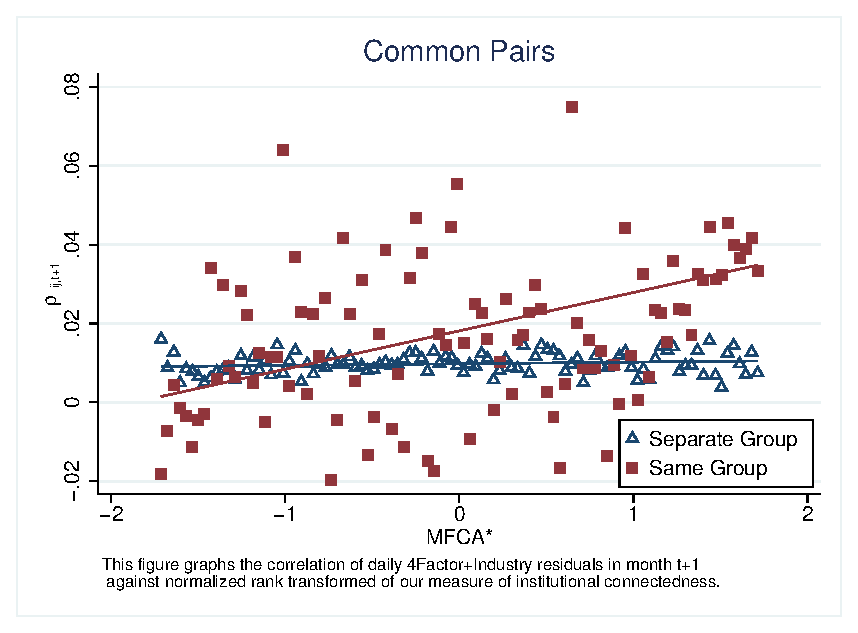
\includegraphics[width=\linewidth]{"Output/mcorr5bg.eps"}     \end{figure}            
			\column{.5\textwidth}
			\begin{figure}
				\centering  
				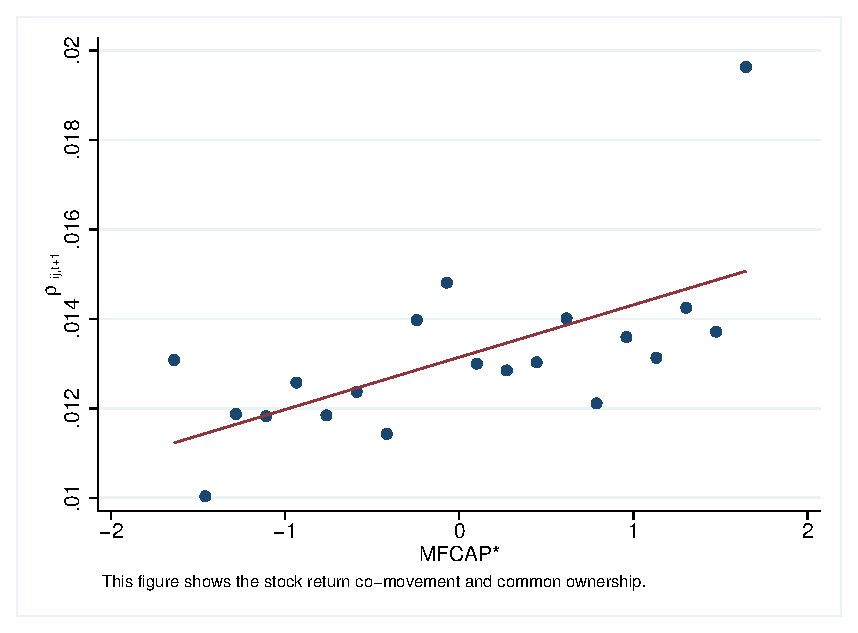
\includegraphics[width=\linewidth]{"Output/mcorr5l.eps"}
			\end{figure}
		\end{columns}
		
		
	\end{frame}
	
	
	
	\begin{frame}{Estimation model}
		\begin{itemize}
			\item Use Fama-MacBeth to estimate this model
			\begin{equation}
\begin{split}
\rho_{ij,t+1} = & \text{ 	}\beta_0 + \beta_1* \text{FCA}^*_{ij,t} + \beta_2* \text{SameGroup}_{ij} \\
 &	+\beta_3* \text{FCA}^*_{ij,t} \times \text{SameGroup}_{ij}   \\
  & + \sum_{k=1} ^{n} \alpha_k*\text{Control}_{ij,t} + \varepsilon_{ij,t+1}
\end{split}
\label{model1}
\end{equation}
			
			\item Estimate the model on a monthly frequency 
			\item Adjust standard errors by Newey and West adjustment with 4 lags ($ 4(70/100)^{\frac{2}{9}} = 3.69 \sim 4 $)
		\end{itemize}
	\end{frame}
	
	\begin{frame}{Model Estimation}{Normalized Rank-Transformed}
			\label{mresult2part1} 
			\begin{table}[htbp]
				\centering
				\resizebox{1\textwidth}{!}{
					{
\def\sym#1{\ifmmode^{#1}\else\(^{#1}\)\fi}
\begin{tabular}{l*{6}{c}}
\hline\hline
                    &\multicolumn{6}{c}{Dependent Variable:  Future Pairs's Comovement}                                                                 \\\cmidrule(lr){2-7}
                    &\multicolumn{1}{c}{(1)}         &\multicolumn{1}{c}{(2)}         &\multicolumn{1}{c}{(3)}         &\multicolumn{1}{c}{(4)}         &\multicolumn{1}{c}{(5)}         &\multicolumn{1}{c}{(6)}         \\
\hline
$ \text{MFCAP*} $   &     0.00600\sym{***}&     0.00328\sym{***}&                     &                     &     0.00104         &    0.000929         \\
                    &      (8.10)         &      (4.87)         &                     &                     &      (1.68)         &      (1.53)         \\
[1em]
SameGroup           &                     &                     &      0.0358\sym{***}&      0.0254\sym{***}&      0.0242\sym{***}&      0.0219\sym{***}\\
                    &                     &                     &      (9.99)         &      (8.45)         &      (8.21)         &      (7.02)         \\
[1em]
SameIndustry        &                     &      0.0267\sym{***}&                     &      0.0216\sym{***}&      0.0212\sym{***}&      0.0215\sym{***}\\
                    &                     &      (7.39)         &                     &      (6.81)         &      (6.72)         &      (6.80)         \\
[1em]
SameBM              &                     &      0.0224\sym{***}&                     &      0.0213\sym{***}&      0.0214\sym{***}&      0.0199\sym{***}\\
                    &                     &      (6.41)         &                     &      (6.09)         &      (6.16)         &      (5.77)         \\
[1em]
SameSize            &                     &      0.0123\sym{**} &                     &      0.0143\sym{***}&      0.0138\sym{***}&      0.0254\sym{***}\\
                    &                     &      (3.24)         &                     &      (3.85)         &      (3.71)         &      (5.56)         \\
[1em]
CrossOwnership      &                     &      0.0600\sym{***}&                     &      0.0300\sym{*}  &      0.0316\sym{*}  &      0.0377\sym{**} \\
                    &                     &      (5.50)         &                     &      (2.36)         &      (2.48)         &      (2.93)         \\
[1em]
Constant            &      0.0142\sym{***}&      0.0204\sym{***}&      0.0103\sym{***}&      0.0187\sym{***}&      0.0188\sym{***}&      0.0280\sym{***}\\
                    &     (12.80)         &      (8.91)         &      (9.42)         &      (7.99)         &      (8.04)         &      (9.43)         \\
\hline
PairType Control    &          No         &          No         &          No         &          No         &          No         &         Yes         \\
Observations        &      389591         &      389591         &      389591         &      389591         &      389591         &      389591         \\
\hline\hline  \end{tabular}}

				}
			\end{table}
			
			
		\end{frame}
	\begin{frame}{Model Estimation}{Normalized Rank-Transformed}
			\label{mresult2part2} 
			\begin{table}[htbp]
				\centering
				\resizebox{1\textwidth}{!}{
					{
\def\sym#1{\ifmmode^{#1}\else\(^{#1}\)\fi}
\begin{tabular}{l*{4}{c}}
\hline\hline
                &\multicolumn{4}{c}{Dependent Variable: Future Pairs's co-movement'}        \\\cmidrule(lr){2-5}
                &\multicolumn{1}{c}{(1)}         &\multicolumn{1}{c}{(2)}         &\multicolumn{1}{c}{(3)}         &\multicolumn{1}{c}{(4)}         \\
\hline
$ \text{MFCAP*} $&  0.00944\sym{***}& 0.000397         & 0.000377         &-0.0000113         \\
                &   (7.24)         &   (0.68)         &   (0.65)         &  (-0.02)         \\
[1em]
Same Group      &                  &                  &  0.00624\sym{**} &  0.00549\sym{*}  \\
                &                  &                  &   (2.81)         &   (2.27)         \\
[1em]
 $ (\text{MFCAP}^*) \times {\text{SameGroup} }  $ &                  &                  &  0.00992\sym{***}&   0.0107\sym{***}\\
                &                  &                  &   (6.49)         &   (6.97)         \\
\hline
Observations    &    58337         &  1607659         &  1665996         &  1665996         \\
Sub-sample      &SameGroup         &   Others         &      All         &      All         \\
Group Effect    &       No         &       No         &       No         &      Yes         \\
Controls        &      Yes         &      Yes         &      Yes         &      Yes         \\
$ R^2 $         &   0.0112         & 0.000577         & 0.000898         &  0.00575         \\
\hline\hline
\multicolumn{5}{l}{\footnotesize \textit{t} statistics in parentheses}\\
\multicolumn{5}{l}{\footnotesize \sym{*} \(p<0.05\), \sym{**} \(p<0.01\), \sym{***} \(p<0.001\)}\\
\end{tabular}
}

				}
			\end{table}
			
			
		\end{frame}
	
	
	\subsection{High level of common ownership}
	
	\begin{frame}{ Future Correlation via $ FCA $}{Discontinuity}\label{Monthly5}
		
		
		
		
		
		\begin{columns}
			\column{.5\textwidth}  
			\begin{figure}   
				\centering
				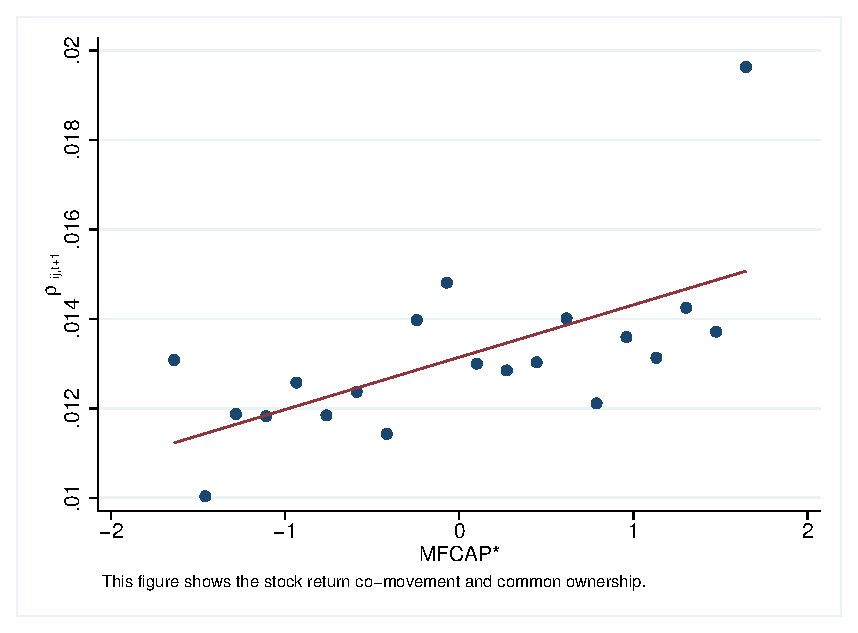
\includegraphics[width=\linewidth]{"Output/mcorr5l.eps"}     \end{figure}            
			\column{.5\textwidth}
			\begin{figure}
				\centering  
				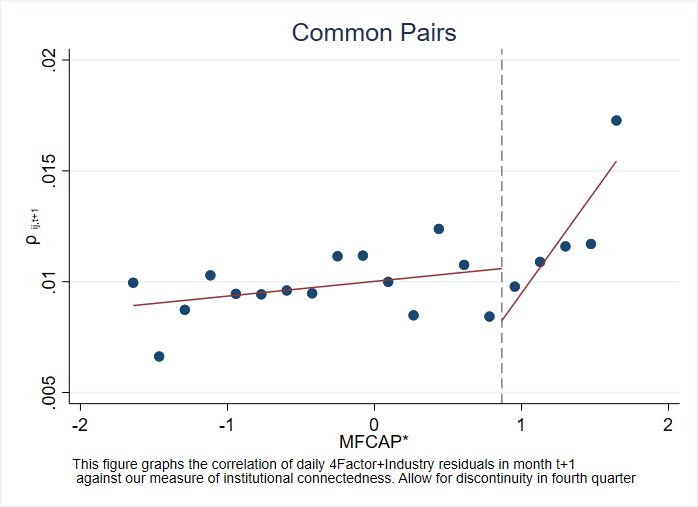
\includegraphics[width=\linewidth]{"Output/Qmcorr5lrd.eps"}
			\end{figure}
		\end{columns}
		\centering
		
		
	\end{frame}
	
	

	
	
%	\begin{frame}{Estimation model}
%		\begin{itemize}
%			\item Use Fama-MacBeth to estimate this model
%			
%			\begin{equation}
\begin{split}
\rho_{ij,t+1} = & \text{ 	}\beta_0 + \beta_1* (\text{FCA}^*_{ij,t} > Q3[\text{FCA}^*_{ij,t}])  + \beta_2 * \text{SameGroup}_{ij}  \\
& +  \beta_3* (\text{FCA}^*_{ij,t} > Q3[\text{FCA}^*_{ij,t}]) \times \text{SameGroup}_{ij}   \\
  & + \sum_{k=1} ^{n} \alpha_k*\text{Control}_{ij,t} + \varepsilon_{ij,t+1}
\end{split}
\label{model2}
\end{equation}
%			
%			\item Estimate that model on a monthly frequency 
%		\end{itemize}
%	\end{frame}
%	
	
	
	
	
	

		
	%
	%
		\begin{frame}{ 4 Factor + Industry Future  Correlation via $ FCA^* $}{Discontinuity \&  Business Groups}\label{Monthly19}
		
		
		
		
		
		\begin{columns}
			\column{.5\textwidth}  
			\begin{figure}   
				\centering
				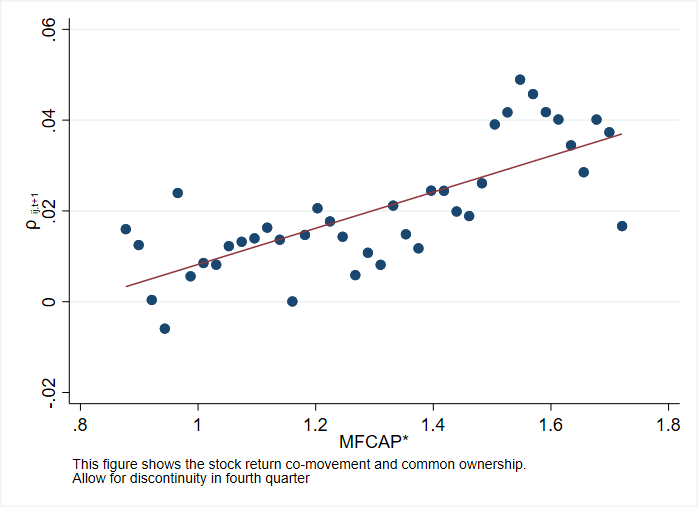
\includegraphics[width=\linewidth]{"Output/Qmcorr5subsample.eps"}     \end{figure}            
			\column{.5\textwidth}
			\begin{figure}
				\centering  
				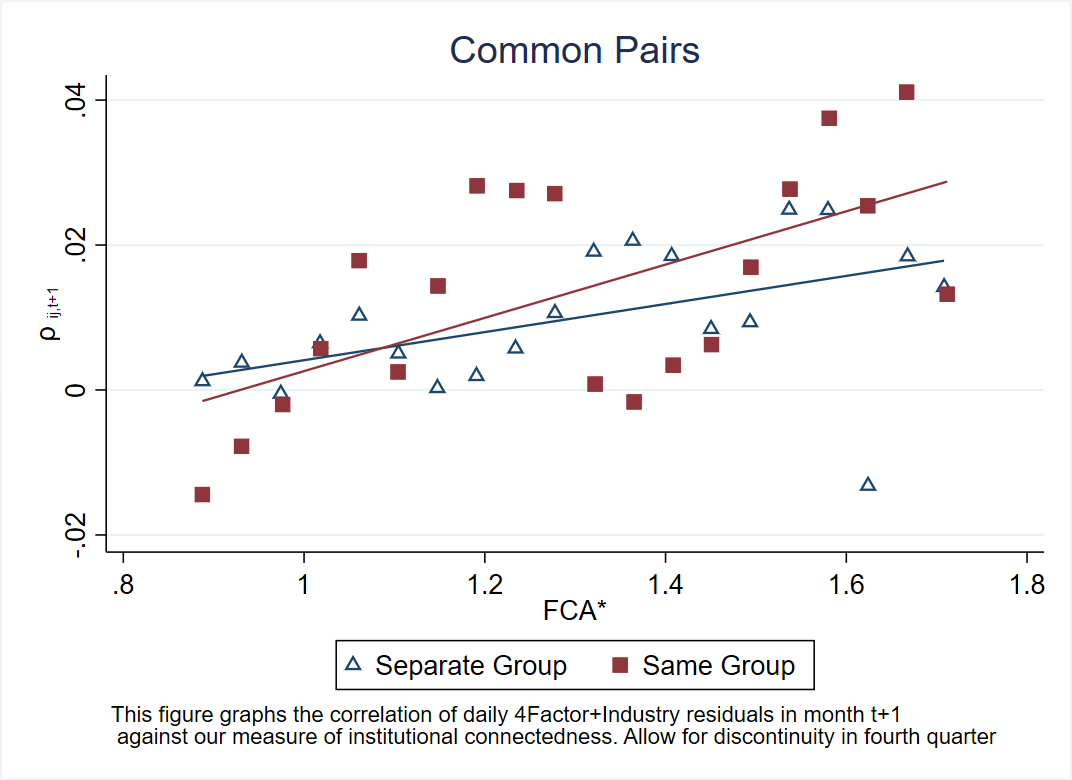
\includegraphics[width=\linewidth]{"Output/Qmcorr5lrdbgsubsample.eps"}
			\end{figure}
		\end{columns}
		\centering
		
		
		
	\end{frame}
		
%\begin{frame}{Forth quarter summary}\label{Monthly22}
%
%\begin{columns}
%\column{.5\textwidth}  
%\begin{figure}   
%\centering
%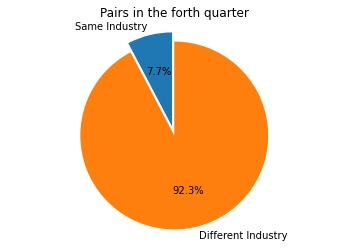
\includegraphics[width=\linewidth]{"Output/sameIndustryinQuarter.eps"}     \end{figure}            
%\column{.5\textwidth}
%\begin{figure}
%\centering  
%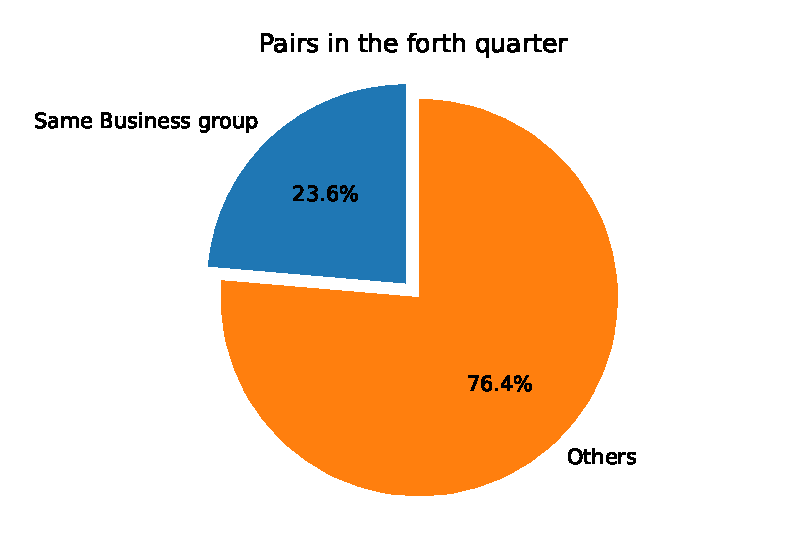
\includegraphics[width=\linewidth]{"Output/sameIBGinQuarter.eps"}
%\end{figure}
%\end{columns}
%\centering
%\end{frame}
		
%\begin{frame}{Forth quarter summary}\label{Monthly21}
%		\begin{figure}
%			\centering  
%			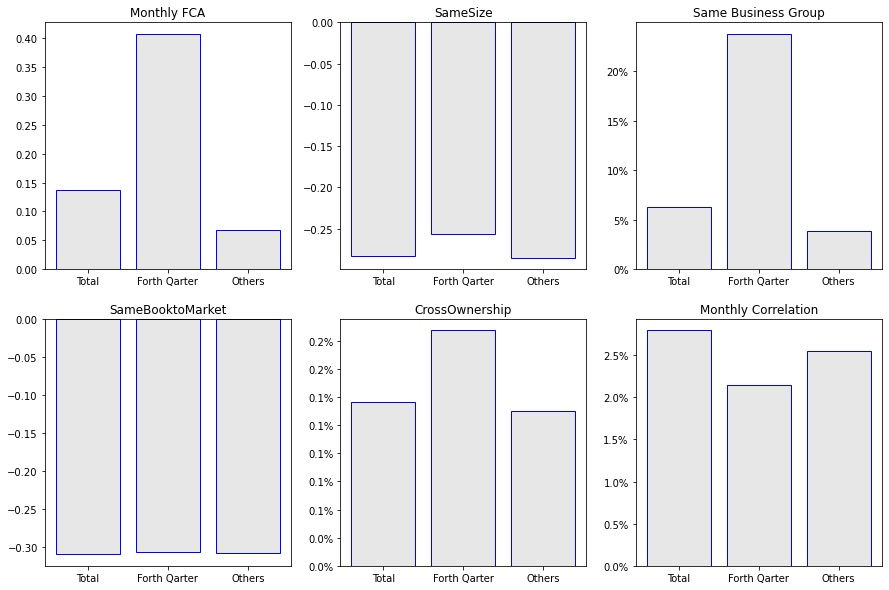
\includegraphics[width=0.9\linewidth]{"Output/QarterSummary.eps"}
%		\end{figure}
%\end{frame}		
		
\begin{frame}{Fama-MacBeth Estimation}{Discontinuity (sub-sample)}
\label{Monthly9} 

\begin{table}[htbp]
	\centering
	\resizebox{0.8\textwidth}{!}{
		{
\def\sym#1{\ifmmode^{#1}\else\(^{#1}\)\fi}
\begin{tabular}{l*{7}{c}}
\hline\hline
                &\multicolumn{7}{c}{Dependent Variable:  Future Pairs's Comovement}                                                                  \\\cmidrule(lr){2-8}
                &\multicolumn{1}{c}{(1)}         &\multicolumn{1}{c}{(2)}         &\multicolumn{1}{c}{(3)}         &\multicolumn{1}{c}{(4)}         &\multicolumn{1}{c}{(5)}         &\multicolumn{1}{c}{(6)}         &\multicolumn{1}{c}{(7)}         \\
\hline
SameGroup       &   0.0254\sym{***}&                  &   0.0249\sym{***}&                  &                  &  0.00477         &  0.00252         \\
                &   (8.45)         &                  &   (8.21)         &                  &                  &   (1.32)         &   (0.66)         \\
[1em]
$ (\text{MFCAP} > \text{Larger than 75th Percentile}) $ &                  &  0.00660\sym{***}& 0.000777         &   0.0230\sym{***}& -0.00258\sym{*}  & -0.00157         &-0.000513         \\
                &                  &   (5.48)         &   (0.73)         &   (7.09)         &  (-2.00)         &  (-1.29)         &  (-0.46)         \\
[1em]
 $ (\text{MFCAP} > Q3[\text{MFCAP}]) \times {\text{SameGroup}} $ &                  &                  &                  &                  &                  &   0.0248\sym{***}&   0.0237\sym{***}\\
                &                  &                  &                  &                  &                  &   (7.24)         &   (7.34)         \\
\hline
Sub-sample      &      All         &      All         &      All         &SameGroup         &   Others         &      All         &      All         \\
Controls        &      Yes         &      Yes         &      Yes         &      Yes         &      Yes         &      Yes         &      Yes         \\
Business Group FE&       No         &       No         &       No         &       No         &       No         &       No         &      Yes         \\
Observations    &   389591         &   389591         &   389591         &    47076         &   342515         &   389591         &   389591         \\
\hline\hline
\multicolumn{8}{l}{\footnotesize \textit{t} statistics in parentheses}\\
\multicolumn{8}{l}{\footnotesize \sym{*} \(p<0.05\), \sym{**} \(p<0.01\), \sym{***} \(p<0.001\)}\\
\end{tabular}
}

	}
\end{table}	
	\end{frame}

\subsection{All pairs}


\begin{frame}{All non-common owner pairs}{regression}
	\begin{table}[htbp]
		\centering
		\resizebox{1\textwidth}{!}{
			{
\def\sym#1{\ifmmode^{#1}\else\(^{#1}\)\fi}
\begin{tabular}{l*{7}{c}}
\hline\hline
                &\multicolumn{7}{c}{Dependent Variable: Future Pairs' co-movement}                                                                   \\\cmidrule(lr){2-8}
                &\multicolumn{1}{c}{(1)}         &\multicolumn{1}{c}{(2)}         &\multicolumn{1}{c}{(3)}         &\multicolumn{1}{c}{(4)}         &\multicolumn{1}{c}{(5)}         &\multicolumn{1}{c}{(6)}         &\multicolumn{1}{c}{(7)}         \\
\hline
SameGroup       &   0.0156\sym{***}&                  &   0.0158\sym{***}&                  &                  &   0.0138\sym{***}&   0.0131\sym{***}\\
                &   (9.84)         &                  &  (10.22)         &                  &                  &   (8.27)         &   (7.68)         \\
[1em]
$ \text{MFCAP*}  $&                  &-0.0000723         &-0.000277         &  0.00169         &-0.000322\sym{*}  &-0.000390\sym{**} &-0.000427\sym{*}  \\
                &                  &  (-0.44)         &  (-1.80)         &   (1.42)         &  (-2.19)         &  (-2.70)         &  (-2.29)         \\
[1em]
 $ (\text{MFCAP}^*) \times {\text{SameGroup} }  $ &                  &                  &                  &                  &                  &  0.00313\sym{**} &  0.00364\sym{**} \\
                &                  &                  &                  &                  &                  &   (2.80)         &   (3.34)         \\
\hline
Controls        &      Yes         &      Yes         &      Yes         &      Yes         &      Yes         &      Yes         &      Yes         \\
Sub-Sample      &    Total         &    Total         &    Total         &SameGroups         &   Others         &    Total         &    Total         \\
Business Group FE&       No         &       No         &       No         &       No         &       No         &       No         &      Yes         \\
Observations    &  6018646         &  6018646         &  6018646         &   114526         &  5904120         &  6018646         &  6018646         \\
\hline\hline
\multicolumn{8}{l}{\footnotesize \textit{t} statistics in parentheses}\\
\multicolumn{8}{l}{\footnotesize \sym{*} \(p<0.05\), \sym{**} \(p<0.01\), \sym{***} \(p<0.001\)}\\
\end{tabular}
}

		}
	\end{table}
\end{frame}


	
	\section{Evidence for correlated trading}
 \subsection{Turnover}
	\begin{frame}{TrunOver}
		\begin{equation*}
			\Delta \text{TurnOver} = \ln(\frac{\text{TurnOver}_{i,t}}{\text{TurnOver}_{i,t-1}}) = 
			\ln({\frac{\text{volume}_{i,t}}{\text{MarketCap}_{i,t}}}) - \ln({\frac{\text{volume}_{i,t-1}}{\text{MarketCap}_{i,t-1}}})
		\end{equation*}
		\pause
\begin{itemize}
	\item 
	\cite{Liquidity2016}
\end{itemize}


	\pause
	\begin{table}[htbp]
		\centering
		\resizebox{0.95\textheight}{!}{
			{
\def\sym#1{\ifmmode^{#1}\else\(^{#1}\)\fi}
\begin{tabular}{l*{4}{c}}
\hline\hline
                    &\multicolumn{4}{c}{Dependent Variable: $\Delta \text{TurnOver}\_{i} $ }                 \\\cmidrule(lr){2-5}
                    &\multicolumn{1}{c}{(1)}         &\multicolumn{1}{c}{(2)}         &\multicolumn{1}{c}{(3)}         &\multicolumn{1}{c}{(4)}         \\
\hline
 $ \Delta \text{TurnOver}_{\text{Market}} $ &       0.416\sym{***}&       0.326\sym{***}&       0.252\sym{***}&       0.228\sym{***}\\
                    &     (12.25)         &      (5.35)         &      (6.41)         &      (4.24)         \\
[1em]
 $ \Delta \text{TurnOver}_{\text{Industry-i}} $ &       0.142\sym{***}&       0.213\sym{***}&      0.0335         &       0.167\sym{**} \\
                    &      (3.79)         &      (6.29)         &      (1.34)         &      (2.87)         \\
[1em]
 $ \Delta \text{TurnOver}_{\text{Group,-i}} $ &                     &                     &       0.330\sym{***}&       0.218\sym{***}\\
                    &                     &                     &     (12.74)         &      (3.80)         \\
\hline
Control             &          No         &         Yes         &          No         &         Yes         \\
Observations        &      854662         &      851772         &      333789         &      331263         \\
$ R^2 $             &       0.285         &       0.543         &       0.433         &       0.712         \\
\hline\hline
\multicolumn{5}{l}{\footnotesize \textit{t} statistics in parentheses}\\
\multicolumn{5}{l}{\footnotesize \sym{*} \(p<0.05\), \sym{**} \(p<0.01\), \sym{***} \(p<0.001\)}\\
\end{tabular}
}

		}
	\end{table}
	
\end{frame}
\begin{frame}{High Beta Group}
	\begin{table}[htbp]
\centering
		\resizebox{0.95\textwidth}{!}{
			\centering
			{
\def\sym#1{\ifmmode^{#1}\else\(^{#1}\)\fi}
\begin{tabular}{l*{4}{c}}
\hline\hline
                &\multicolumn{4}{c}{Dependent Variable: Future Pairs's co-movement}         \\\cmidrule(lr){2-5}
                &\multicolumn{1}{c}{(1)}         &\multicolumn{1}{c}{(2)}         &\multicolumn{1}{c}{(3)}         &\multicolumn{1}{c}{(4)}         \\
\hline
Same Group      &   0.0180\sym{***}&   0.0178\sym{***}&   0.0118\sym{***}&   0.0133\sym{***}\\
                &   (8.45)         &   (8.25)         &   (5.26)         &   (5.81)         \\
[1em]
HighBetaGroup   &                  & 0.000988         & 0.000808         & 0.000485         \\
                &                  &   (1.35)         &   (1.09)         &   (0.44)         \\
[1em]
$ {\text{HighBetaGroup} } \times {\text{SameGroup} }  $ &                  &                  &  0.00702\sym{*}  &  0.00477         \\
                &                  &                  &   (2.00)         &   (1.38)         \\
\hline
Observations    &  1665996         &  1665996         &  1665996         &  1665996         \\
Group Effect    &       No         &       No         &       No         &      Yes         \\
Pair Size FE    &      Yes         &      Yes         &      Yes         &      Yes         \\
Sub-sample      &    Total         &    Total         &    Total         &    Total         \\
Controls        &      Yes         &      Yes         &      Yes         &      Yes         \\
$ R^2 $         &  0.00120         &  0.00133         &  0.00141         &  0.00594         \\
\hline\hline
\multicolumn{5}{l}{\footnotesize \textit{t} statistics in parentheses}\\
\multicolumn{5}{l}{\footnotesize \sym{*} \(p<0.05\), \sym{**} \(p<0.01\), \sym{***} \(p<0.001\)}\\
\end{tabular}
}

		}
		\label{Turnovercrosssection}
	\end{table}
\end{frame}

\begin{frame}{Pairwise correlations in  turnover}
	\begin{table}[htbp]
		\centering
		\resizebox{0.95\textwidth}{!}{
			\centering
			{
\def\sym#1{\ifmmode^{#1}\else\(^{#1}\)\fi}
\begin{tabular}{l*{7}{c}}
\hline\hline
                    &\multicolumn{7}{c}{Dependent Variable:  Monthly Correlation of Delta turnover}                                                                           \\\cmidrule(lr){2-8}
                    &\multicolumn{1}{c}{(1)}         &\multicolumn{1}{c}{(2)}         &\multicolumn{1}{c}{(3)}         &\multicolumn{1}{c}{(4)}         &\multicolumn{1}{c}{(5)}         &\multicolumn{1}{c}{(6)}         &\multicolumn{1}{c}{(7)}         \\
\hline
SameGroup           &      0.0180\sym{***}&                     &      0.0173\sym{***}&                     &                     &      0.0150\sym{***}&      0.0168\sym{***}\\
                    &      (6.19)         &                     &      (5.53)         &                     &                     &      (4.89)         &      (5.40)         \\
[1em]
$ \text{MFCAP*} $   &                     &     0.00219\sym{**} &    0.000543         &     0.00115         &    0.000372         &    0.000363         &   -0.000413         \\
                    &                     &      (2.84)         &      (0.69)         &      (0.57)         &      (0.41)         &      (0.40)         &     (-0.37)         \\
[1em]
 $ (\text{MFCAP}^*) \times {\text{SameGroup} }  $ &                     &                     &                     &                     &                     &     0.00260         &     0.00296         \\
                    &                     &                     &                     &                     &                     &      (1.03)         &      (1.19)         \\
\hline
Sub-sample          &         All         &         All         &         All         &   SameGroup         &      Others         &         All         &         All         \\
Business Group FE   &          No         &          No         &          No         &          No         &          No         &          No         &         Yes         \\
Observations        &      294864         &      294864         &      294864         &       37076         &      257788         &      294864         &      294864         \\
\hline\hline
\multicolumn{8}{l}{\footnotesize \textit{t} statistics in parentheses}\\
\multicolumn{8}{l}{\footnotesize \sym{*} \(p<0.05\), \sym{**} \(p<0.01\), \sym{***} \(p<0.001\)}\\
\end{tabular}
}

		}
		\label{mresult2-turnover}
	\end{table}
\end{frame}
	\begin{frame}{Turn over and Comovement}
		\begin{table}[htbp]
			\centering
			\resizebox{\textheight}{!}{
				{
\def\sym#1{\ifmmode^{#1}\else\(^{#1}\)\fi}
\begin{tabular}{l*{5}{c}}
\hline\hline
                &\multicolumn{5}{c}{Dependent Variable: Future Pairs's co-movement}                            \\\cmidrule(lr){2-6}
                &\multicolumn{1}{c}{(1)}         &\multicolumn{1}{c}{(2)}         &\multicolumn{1}{c}{(3)}         &\multicolumn{1}{c}{(4)}         &\multicolumn{1}{c}{(5)}         \\
\hline
Same Group      &   0.0263\sym{***}&   0.0250\sym{***}&   0.0380\sym{***}&   0.0244\sym{**} &   0.0256\sym{***}\\
                &   (3.79)         &   (3.55)         &   (5.82)         &   (3.33)         &   (4.02)         \\
[1em]
 $ {\rho\_t(\text{Turnover})} $ &  0.00475\sym{***}&  0.00419\sym{***}&  0.00474\sym{***}&  0.00383\sym{***}&  0.00493\sym{***}\\
                &   (9.75)         &   (8.55)         &   (4.65)         &   (4.64)         &   (4.66)         \\
[1em]
 $ {\rho\_t} $   &   0.0249\sym{***}&   0.0248\sym{***}&   0.0248\sym{***}&   0.0252\sym{***}&   0.0243\sym{***}\\
                &  (11.12)         &  (11.10)         &  (11.03)         &  (10.64)         &   (8.58)         \\
[1em]
$ {\text{SameGroup} \times  {\rho\_t(\text{Turnover})} } $ &                  &   0.0172\sym{***}& -0.00936         &   0.0224\sym{***}&  -0.0114         \\
                &                  &   (3.63)         &  (-0.84)         &   (4.42)         &  (-1.04)         \\
[1em]
BigGroup        &                  &                  & -0.00186         &                  &                  \\
                &                  &                  &  (-1.99)         &                  &                  \\
[1em]
$ {\text{BigGroup} } \times {\text{SameGroup} }  $ &                  &                  &  -0.0151\sym{*}  &                  &                  \\
                &                  &                  &  (-2.43)         &                  &                  \\
[1em]
$ {\text{BigGroup} } \times  {\rho\_t(\text{Turnover})}  $ &                  &                  &-0.000833         &                  &                  \\
                &                  &                  &  (-0.53)         &                  &                  \\
[1em]
$ {\text{BigGroup}}\times{\text{SameGroup}}\times  {\rho\_t(\text{Turnover})}$ &                  &                  &   0.0317\sym{*}  &                  &                  \\
                &                  &                  &   (2.64)         &                  &                  \\
\hline
Observations    &  1459585         &  1459585         &  1459585         &   957316         &   502269         \\
Controls        &      Yes         &      Yes         &      Yes         &      Yes         &      Yes         \\
Pari Size FE    &      Yes         &      Yes         &      Yes         &      Yes         &      Yes         \\
SubSample       &      All         &      All         &      All         &Big Groups         &   Others         \\
$ R^2$          &  0.00244         &  0.00255         &  0.00302         &  0.00307         &  0.00396         \\
\hline\hline
\multicolumn{6}{l}{\footnotesize \textit{t} statistics in parentheses}\\
\multicolumn{6}{l}{\footnotesize \sym{*} \(p<0.05\), \sym{**} \(p<0.01\), \sym{***} \(p<0.001\)}\\
\end{tabular}
}

			}
		\end{table}
	\end{frame}

	
	
\subsection{Institutional Imbalance}
\begin{frame}{Ins Imbalance}

\begin{itemize}
	\item \cite{seasholes2007predictable}
	
		\begin{equation*}
			Imbalance_{ins} = \frac{Buy_{ins} - Sell_{ins}}{Buy_{ins} + Sell_{ins}}
		\end{equation*}
	\begin{table}[htbp]
		\centering
		\resizebox{0.8\textwidth}{!}{
			\begin{tabular}{lrrrrrrrr}
\toprule
{} &  Group $\times$ Month &   mean &    std &  min &    25\% &    50\% &    75\% &  max \\
Grouped   &                       &        &        &      &        &        &        &      \\
\midrule
Ungrouped &                 20197 &  0.010 &  0.630 & -1.0 & -0.474 &  0.016 &  0.479 &  1.0 \\
Grouped   &                 12021 & -0.041 &  0.581 & -1.0 & -0.462 & -0.009 &  0.341 &  1.0 \\
\bottomrule
\end{tabular}

		}
		\label{tab:ImbalanceInsMeanSummary}
	\end{table}
		
	
	
\end{itemize}

\end{frame}


\begin{frame}{Ins Imbalance std}
%\begin{columns}
%	\column{0.5\linewidth}
	\begin{table}[htbp]
		\centering
		\resizebox{0.85\textwidth}{!}{
			\begin{tabular}{lcccccccc}
\toprule
{} &  Group $\times$ Month &   mean &    std &   min &    25\% &    50\% &    75\% &    max \\
Grouped   &                       &        &        &       &        &        &        &        \\
\midrule
Ungrouped &                    72 &  0.624 &  0.054 &  0.48 &  0.601 &  0.631 &  0.655 &  0.735 \\
Grouped   &                  2057 &  0.503 &  0.251 &  0.00 &  0.337 &  0.503 &  0.647 &  1.414 \\
\bottomrule
\end{tabular}

		}
		\label{tab:ImbalanceInsStdSummary}
	\end{table}


%	\column{0.5\linewidth}

\begin{figure}[htbp]
	\centering
	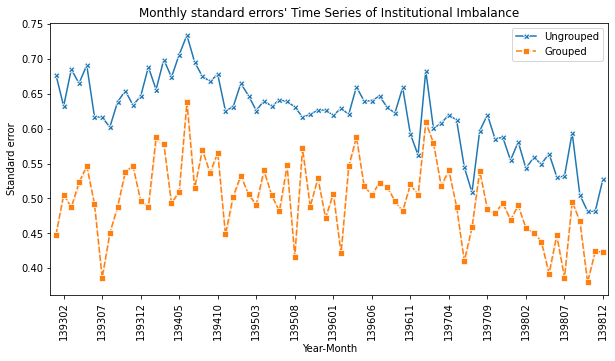
\includegraphics[width=0.85\linewidth]{Output/GroupedInsSTD.eps}
	\label{fig:GroupedInsSTD}
\end{figure}
%\end{columns}
\end{frame}
\begin{frame}{Low Ins Imbalance Group}


				\begin{table}[htbp]
			\centering
			\resizebox{0.8\textwidth}{!}{
				{
\def\sym#1{\ifmmode^{#1}\else\(^{#1}\)\fi}
\begin{tabular}{l*{6}{c}}
\hline\hline
                    &\multicolumn{6}{c}{Dependent Variable:  Future Pairs's Comovement}                                                                 \\\cmidrule(lr){2-7}
                    &\multicolumn{1}{c}{(1)}         &\multicolumn{1}{c}{(2)}         &\multicolumn{1}{c}{(3)}         &\multicolumn{1}{c}{(4)}         &\multicolumn{1}{c}{(5)}         &\multicolumn{1}{c}{(6)}         \\
\hline
SameGroup           &      0.0208\sym{***}&      0.0206\sym{***}&                     &                     &     0.00619         &     0.00630\sym{*}  \\
                    &      (7.91)         &      (7.94)         &                     &                     &      (1.95)         &      (2.04)         \\
[1em]
LowImbalanceStd     &                     &    -0.00144         &      0.0282\sym{***}&    -0.00724\sym{***}&    -0.00610\sym{***}&    -0.00267         \\
                    &                     &     (-1.15)         &      (6.06)         &     (-5.74)         &     (-4.87)         &     (-1.85)         \\
[1em]
 $ \text{LowImbalanceStd} \times {\text{SameGroup} } $ &                     &                     &                     &                     &      0.0358\sym{***}&      0.0325\sym{***}\\
                    &                     &                     &                     &                     &      (8.57)         &      (7.48)         \\
\hline
Sub-sample          &       Total         &       Total         &   SameGroup         &      Others         &       Total         &       Total         \\
Business Group FE   &          No         &          No         &          No         &          No         &          No         &         Yes         \\
Observations        &      354209         &      354209         &       43274         &      310935         &      354209         &      354209         \\
\hline\hline
\multicolumn{7}{l}{\footnotesize \textit{t} statistics in parentheses}\\
\multicolumn{7}{l}{\footnotesize \sym{*} \(p<0.05\), \sym{**} \(p<0.01\), \sym{***} \(p<0.001\)}\\
\end{tabular}
}

			}
		\end{table}
	
	\end{frame}

	
	\section{Conclusion}
	
	\begin{frame}{Conclusion}
		\begin{itemize}
			
			\item We derive a measure that captures the extent of common ownership distribution.
			
			
			\item Direct common ownership can affect firms' co-movement
			\item 
			Firms in the business groups co-move more than other pairs
			\item Direct common ownership only matters for firms in the business groups
			\item Firms in the same business group trade in one way
			
		\end{itemize}
	\end{frame}
	
	\tiny
	\begin{frame}[allowframebreaks]{References}
		
		{		
			\bibliographystyle{apalike}
			\bibliography{Ref}
		}
	\end{frame}
	
	\normalsize
	
	
	\color{black}
	\appendix
	
	
	
	
	
	
	\section{Appendix I}
	\begin{frame}{Measuring Common Ownership}{Proof}\label{Proof}
		
		
		\begin{itemize}
			\item  If two stocks in pair have n mutual owner, which total market cap divides them equally, the mentioned indexes equal n.
			
			\begin{itemize}
				
				\item Each holder owns $ 1/n $ of each firm.
				\item Firm's market cap is $ \alpha_1 $ and $ \alpha_2 $:
				\item So for each holder of firms we have $ S^f_{i,t}P_{i,t} = \alpha_i $
				\item    SQRT
				\begin{align*}
					[  \frac{\sum_{f=1}^{n} \sqrt{\alpha_1/n}+\sum_{f=1}^{n} \sqrt{\alpha_2/n}}{\sqrt{\alpha_1} + \sqrt{\alpha_2}}]^2 
					= [\frac{\sqrt{n}(\sqrt{\alpha_1} +\sqrt{\alpha_2 })}{\sqrt{\alpha_1} + \sqrt{\alpha_2}}]^2 = n
				\end{align*}                  
				
				
				\item	 Quadratic
				\begin{align*}
					[  \frac{\sum_{f=1}^{n} {(\alpha_1/n)^2}+\sum_{f=1}^{n} {(\alpha_2/n)^2}}{\alpha_1^2 +{\alpha_2}^2}]^{-1} 
					=[\frac{{\alpha_1^2 + \alpha_2^2 }}{n(\alpha_1^2 + \alpha_2^2)}]^{-1} = n
				\end{align*}
				
			\end{itemize}
		\end{itemize}
		
		\hfill
		\hyperlink{Intuition}{\beamerbutton{Back}}
		
	\end{frame}
	
			
			\begin{frame}{Measuring Common-ownership}\label{Intuition}
				\cite{AntonPolk}
				\begin{align*}
					\boxed{FCAP_{ij,t} = \frac{\sum_{f = 1}^{F} (S^f_{i,t}P_{i,t}+S^f_{j,t}P_{j,t})}{S_{i,t}P{i,t} + S_{j,t}P{j,t}}}
				\end{align*}
			\pause
				\begin{columns}
					\column{.5\textwidth}     
					\centering
					SQRT
					\begin{align*}
						\boxed{              [\frac{\sum_{f =1}^{F}(\sqrt{S^f_{i,t}P_{i,t}}+\sqrt{S^f_{j,t}P_{j,t}})}{\sqrt{S_{i,t}P{i,t}} + \sqrt{S_{j,t}P{j,t}}}]^2 }
					\end{align*}     
				             
					\column{.5\textwidth}
					\centering  
					Quadratic
					\begin{align*}
						\boxed{    [{\frac{\sum_{f = 1}^{F}[(S^f_{i,t}P_{i,t})^2+(S^f_{j,t}P_{j,t})^2]}{(S_{i,t}P{i,t})^2 + (S_{j,t}P{j,t})^2}}]^{-1}}
					\end{align*}
				\end{columns}
			\pause
				\begin{block}{Intuition}
					If for a pair of stocks with n mutual owners, all owners have even shares of each firm's market cap, then the proposed indexes will be equal to n.
					\hyperlink{Proof}{\beamerbutton{Proof}}
				\end{block}
				
			\end{frame}
			
			
			
			
			\begin{frame}{Measuring Common Ownership}{Example}
				
				\begin{figure}[htbp]
					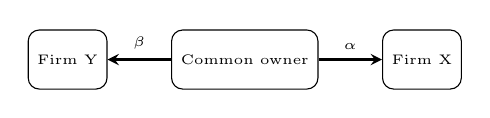
\begin{tikzpicture}[node distance=1cm]
						
						
						\node (Firm) [startstop3] {\tiny Firm X};
						\node (Firm2) [startstop3,right of = Firm , yshift=0cm , xshift=-5.5cm ] {\tiny Firm Y};
						\node (Owner) [startstop3,right of = Firm , yshift=0cm , xshift=-3.25cm ] {\tiny Common owner };
						
						\draw[arrow] (Owner) -- node[sloped, anchor=center, above] {\tiny $ \alpha $} (Firm) ;
						
					\draw[arrow] (Owner) -- node[sloped, anchor=center, above] {\tiny $ \beta $} (Firm2) ;
						%
						%\node() at (3,0)
						%    {$ \alpha + \beta = 100 $}; 
					\end{tikzpicture}
					
				\end{figure}\bigskip
				\pause
				\begin{itemize}
					\item[] For better observation, assume that 
					\begin{itemize}
						\item $ \alpha + \beta = 100 $\\
						\item both firm have equal market cap
					\end{itemize} 
				\end{itemize}
			\pause
				\begin{figure}[htbp]
					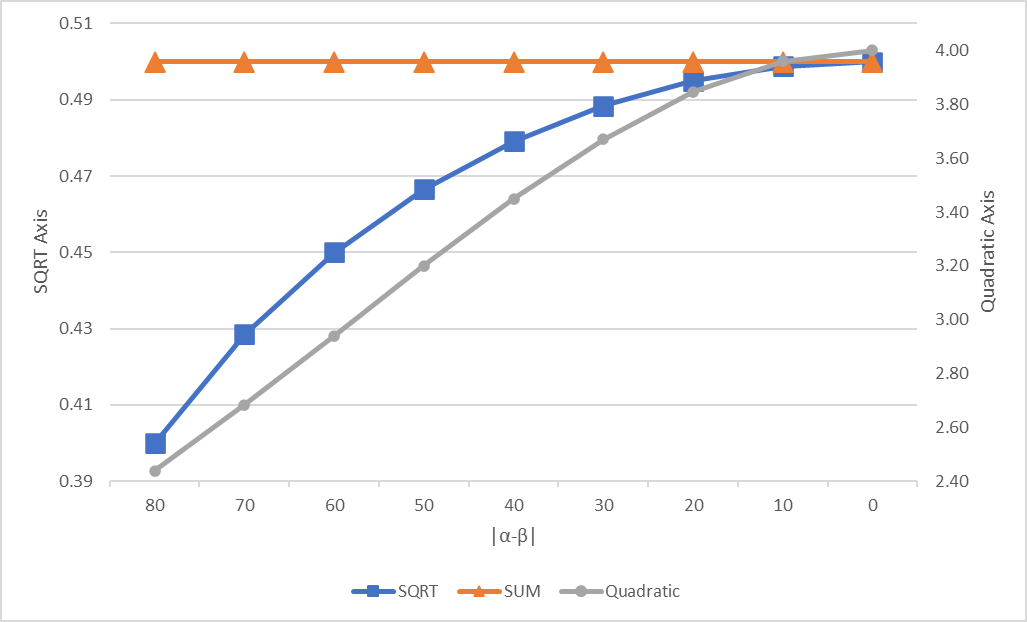
\includegraphics[width=0.47\linewidth]{1.png}
					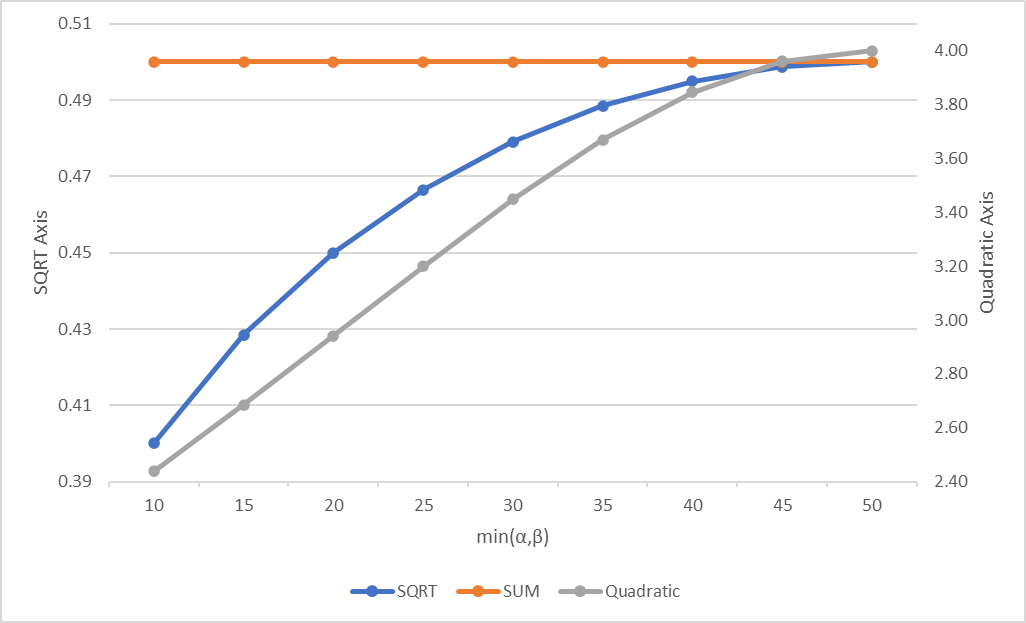
\includegraphics[width=0.47\linewidth]{2.png}
					\captionsetup{labelformat=empty}
					\caption{\scriptsize Comparison of three methods for calculating common ownership}
				\end{figure}
			\end{frame}
			
			
			\begin{frame}{Measuring Common Ownership}{Example of three common owner}
				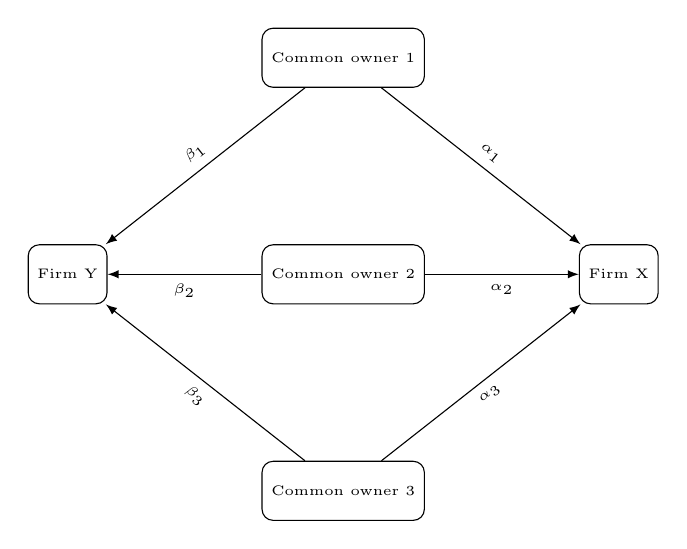
\begin{tikzpicture}[node distance=1cm]
					
					
					\node (Firm) [startstop3] {\tiny Firm X};
					\node (Firm2) [startstop3,right of = Firm , yshift=0cm , xshift=-8cm ] {\tiny Firm Y};
					\pause
					\node (Owner) [startstop3,above of = Firm , yshift=1.75cm , xshift=-3.5cm ] {\tiny Common owner 1 };
		
					
					\node (Owner2) [startstop3,right of = Firm , yshift= 0 , xshift=-4.5cm ] {\tiny Common owner 2 };
					
					\node (Owner3) [startstop3,below of = Firm , yshift=-1.75cm , xshift=-3.5cm ] {\tiny Common owner 3 };
					
					\pause
					
					
					
					\draw [-latex] (Owner) to [bend right =0]  node[sloped, anchor=center, above] {\tiny $ \beta_1 $} (Firm2);
					
					\draw [-latex] (Owner) to [bend left =0]  node[sloped, anchor=center, above] {\tiny $ \alpha_1 $} (Firm);
					
					\pause
					
					\draw [-latex] (Owner2) to [bend right =0]  node[sloped, anchor=center, below] {\tiny $ \beta_2 $} (Firm2);
					
					\draw [-latex] (Owner2) to [bend left =0]  node[sloped, anchor=center, below] {\tiny $ \alpha_2 $} (Firm);
					
					
					
					\draw [-latex] (Owner3) to [bend left =0]  node[sloped, anchor=center, below] {\tiny$ \beta_3 $} (Firm2);
					
					\draw [-latex] (Owner3) to [bend right =0]  node[sloped, anchor=center, below] {\tiny $ \alpha_3 $} (Firm);
					
					
					
				\end{tikzpicture}
				
			\end{frame}
			
			
			\begin{frame}{Measuring Common Ownership}{Example of three common owner}
				\begin{table}[htbp]
					\centering
					\resizebox{0.9\textwidth}{!}
					{
						    \begin{tabular}{cccccccc}
    \hline\hline
        Ownership  & Type I & Type II & Type III & Type IV & Type V & Type VI & Type VII \\
          \hline
    $ \alpha_1 $    & 1/3 &20      &  10   & 20    & 10    & 5     & 1  \\
    $ \beta_1 $    & 1/3  & 10    & 10   & 20    & 10    & 5     & 1  \\
    $ \alpha_2 $    & 1/3  & 10    & 80    & 20    & 10    & 5     & 1 \\
    $ \beta_2 $    & 1/3  & 20    & 80    & 20    & 10    & 5     & 1  \\
    $ \alpha_3 $    & 1/3  & 70    & 10    & 20    & 10    & 5     & 1 \\
    $ \beta_3 $    & 1/3  & 70    & 10   & 20    & 10    & 5     & 1  \\
    \hline
    SQRT  & 3     &  2.56  & 2.33 & 1.8   & 0.9   & 0.45  & 0.09 \\
    SUM   & 1     & 1     & 1     & 0.6   & 0.3   & 0.15  & 0.03 \\
    Quadratic & 3     & 1.85  & 1.52  & 8.33  & 33.33 & 133.33 & 3333.33 \\
 
    \hline\hline
    \end{tabular}%
					}
				\end{table}
				
			\end{frame}
			
			
			
			\begin{frame}{Measuring Common Ownership}{Comparison}
				\begin{itemize}
					\item For better comparison we relax previous assumptions:
					\begin{itemize}
						\item Two Firms with different market caps.
					\end{itemize}
				\end{itemize}
				\resizebox{0.7\textwidth}{!}
				{
					          \scriptsize
    \begin{tabular}{ccccccc}
    \hline\hline
  & \multicolumn{6}{c}{\tiny($ \alpha_1 $,$ \beta_1 $),($ \alpha_2 $,$ \beta_2 $) }\\ \cmidrule(lr){2-7}
               & \multicolumn{2}{c}{\tiny(10,40),(10,40)} & \multicolumn{2}{c}{\tiny(15,35),(15,35)} & \multicolumn{2}{c}{\tiny(20,30),(20,30)} \\ \cmidrule(lr){2-3}\cmidrule(lr){4-5}\cmidrule(lr){6-7}
    \tiny $ \frac{\text{MarketCap}_x}{\text{MarketCap}_y} $     &\tiny SQRT  & \tiny SUM   &\tiny SQRT  &\tiny SUM   &\tiny SQRT  &\tiny SUM \\ 
     \hline\addlinespace

         1     & 0.90  & 0.50  & 0.96  & 0.50  & 0.99  & 0.50 \\
         2     & 0.80  & 0.40  & 0.89  & 0.43  & 0.96  & 0.47 \\
         3     & 0.75  & 0.35  & 0.85  & 0.40  & 0.94  & 0.45 \\
         4     & 0.71  & 0.32  & 0.83  & 0.38  & 0.92  & 0.44 \\
         5     & 0.69  & 0.30  & 0.81  & 0.37  & 0.91  & 0.43 \\
         6     & 0.67  & 0.29  & 0.80  & 0.36  & 0.91  & 0.43 \\
         7     & 0.65  & 0.28  & 0.79  & 0.35  & 0.90  & 0.43 \\
         8     & 0.64  & 0.27  & 0.78  & 0.34  & 0.90  & 0.42 \\
         9     & 0.63  & 0.26  & 0.77  & 0.34  & 0.89  & 0.42 \\
         10    & 0.62  & 0.25  & 0.76  & 0.34  & 0.89  & 0.42 \\
     
    \hline\hline
    \end{tabular}
				}
				
				
			\end{frame}
			
			
			\begin{frame}{Measuring Common Ownership}{Comparison}
				\begin{figure}[htbp]
					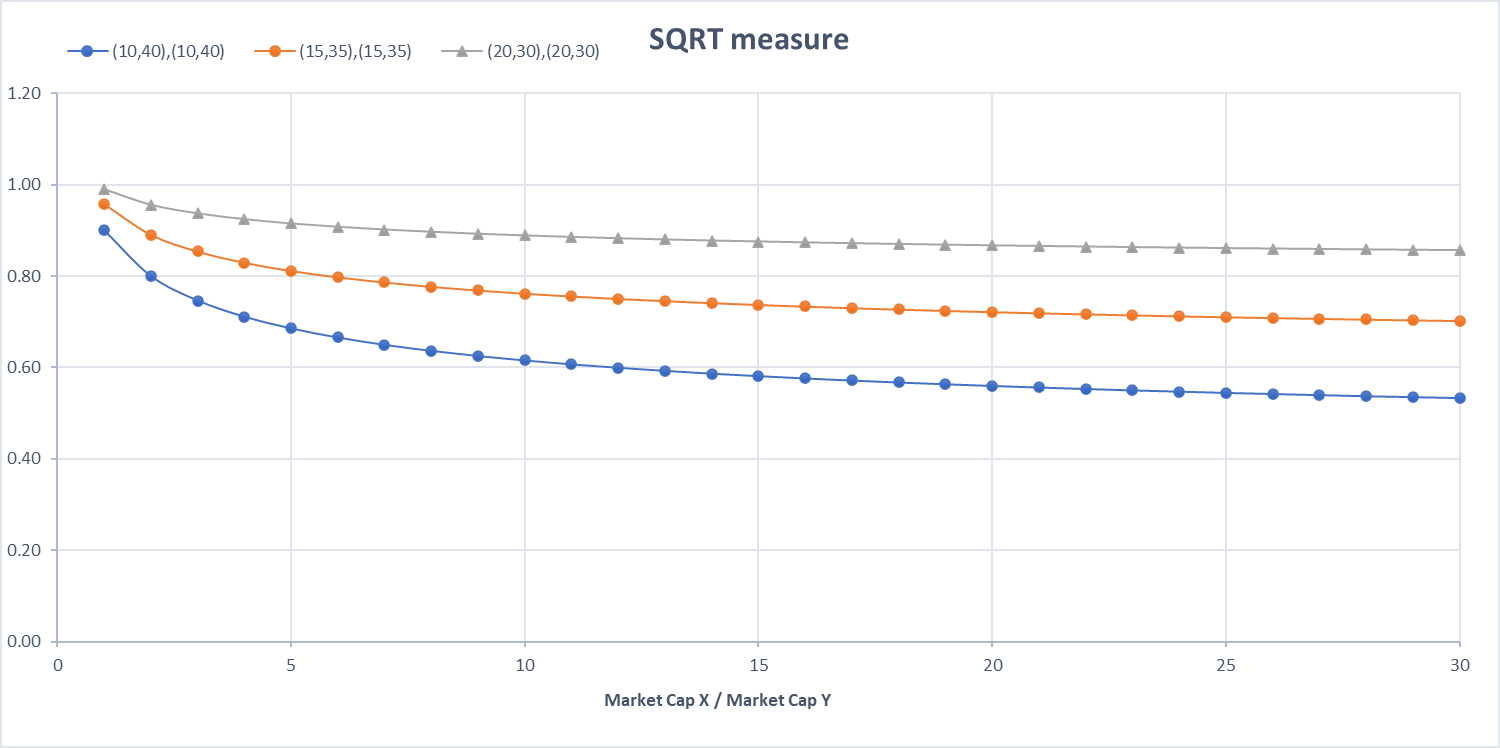
\includegraphics[width=0.47\linewidth]{3.png}
					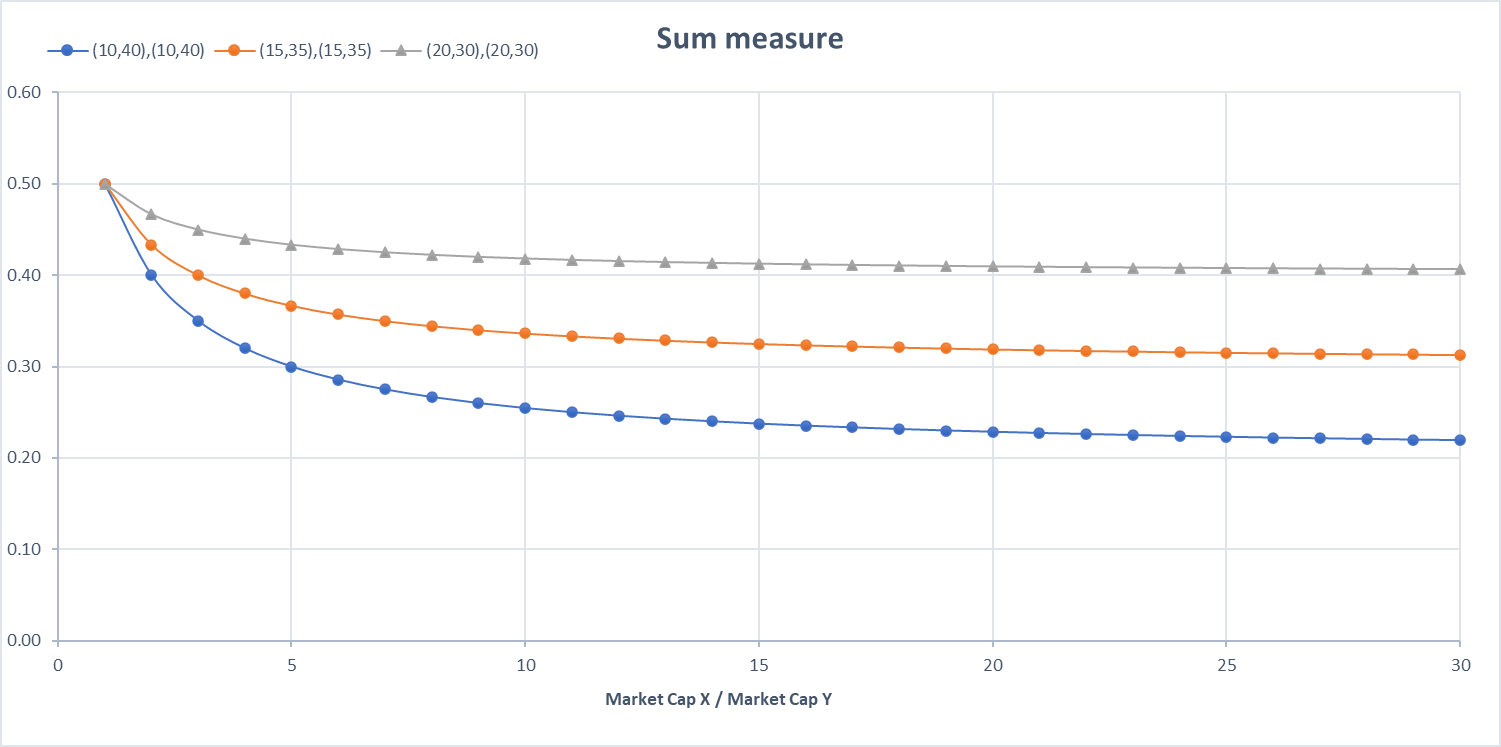
\includegraphics[width=0.47\linewidth]{4.png}
					\captionsetup{labelformat=empty}
					\caption{\scriptsize Comparison of two methods for calculating common ownership}
				\end{figure}
				\begin{block}{Conclusion}
					We use the SQRT measure because it has an acceptable variation and has fair values at a lower level of aggregate common ownership. 
				\end{block}
			\end{frame}
		\begin{frame}{Common Ownership measure}	
			\begin{table}[htbp]
						\centering
					\resizebox{1\textwidth}{!}{
						{
\def\sym#1{\ifmmode^{#1}\else\(^{#1}\)\fi}
\begin{tabular}{l*{8}{c}}
\hline\hline
                &\multicolumn{8}{c}{Dependent Variable: Future Monthly Correlation of 4F+Industry Residuals}                                                            \\\cmidrule(lr){2-9}
                &\multicolumn{1}{c}{(1)}         &\multicolumn{1}{c}{(2)}         &\multicolumn{1}{c}{(3)}         &\multicolumn{1}{c}{(4)}         &\multicolumn{1}{c}{(5)}         &\multicolumn{1}{c}{(6)}         &\multicolumn{1}{c}{(7)}         &\multicolumn{1}{c}{(8)}         \\
\hline
Common Ownership Measure&  0.00370\sym{***}&  0.00325\sym{***}&  0.00155\sym{*}  &  0.00109         & 0.000333         &-0.000105         & 0.000550         & 0.000283         \\
                &   (5.58)         &   (4.97)         &   (2.61)         &   (1.84)         &   (0.54)         &  (-0.17)         &   (1.07)         &   (0.58)         \\
[1em]
SameGroup       &                  &                  &   0.0229\sym{***}&   0.0234\sym{***}&   0.0100\sym{**} &   0.0103\sym{**} &  0.00626         &  0.00668         \\
                &                  &                  &   (7.89)         &   (7.93)         &   (3.26)         &   (3.17)         &   (1.79)         &   (1.79)         \\
[1em]
 $ \text{\small Common Ownership Measure} \times {\text{SameGroup} }$ &                  &                  &                  &                  &   0.0134\sym{***}&   0.0135\sym{***}&   0.0127\sym{***}&   0.0126\sym{***}\\
                &                  &                  &                  &                  &   (9.47)         &  (10.65)         &   (9.23)         &   (9.71)         \\
\hline
Observations    &   398818         &   398818         &   398818         &   398818         &   398818         &   398818         &   398818         &   398818         \\
Group FE        &       No         &       No         &       No         &       No         &       No         &       No         &      Yes         &      Yes         \\
Measurement     &      Sum         &      Sum         &      Sum         &      Sum         &      Sum         &     SQRT         &      Sum         &     SQRT         \\
$ R^2 $         &  0.00433         &  0.00427         &  0.00518         &  0.00515         &  0.00554         &  0.00551         &   0.0182         &   0.0182         \\
\hline\hline
\multicolumn{9}{l}{\footnotesize \textit{t} statistics in parentheses}\\
\multicolumn{9}{l}{\footnotesize \sym{*} \(p<0.05\), \sym{**} \(p<0.01\), \sym{***} \(p<0.001\)}\\
\end{tabular}
}
}
			\end{table}
		\end{frame}	
		
	
	\section{Appendix II}
	\begin{frame}{Main Effect}\label{maineffect}
		
		\begin{itemize}
			\item \color{cyan} Common-ownership and comovement effect 
			\\
			\scriptsize
			\normalcolor
			[\cite{AntonPolk}]
			\\  \tiny 
			Stocks sharing many common investors tend to comove more strongly with each other in the future than otherwise similar stocks.
			
			\normalsize
			\item \color{cyan} Common-ownership and liquidity demand 
			\\
			\scriptsize
			\normalcolor 
			[\cite{Liquidity2016}, Pastor and Stambaugh (2003), Acharya and Pedersen (2005)]
			\normalsize
			\\
			\tiny Commonality in stock liquidity is likely driven by correlated trading among a given stock’s investors.
			Commonality in liquidity is important because it can influence expected returns 
			
			\normalsize
			
			
			
			\item \color{cyan} Trading needs and comovement 
			\\
			\scriptsize
			\normalcolor
			[\cite{greenwood2011stock}]
			\normalsize
			\\  
			\tiny   If the investors of mutual funds have correlated trading needs, the stocks that are held by mutual funds can comove even without any portfolio overlap of the funds themselves 
			
			\normalsize
			
			
			
			\item \color{cyan} Stock price synchronicity and poor corporate governance 
			\\
			\scriptsize
			\normalcolor
			[\cite{boubaker2014large}, \cite{khanna2009synchronicity}, Morck et al. (2000)]
			\normalsize
			\\  
			\tiny   Stock price synchronicity has been attributed to poor corporate governance and a lack of firm-level transparency. On the other hand, better law protection encourages informed trading, which facilitates the incorporation of firm-specific information into stock prices, leading to lower synchronicity 
			
			\normalsize
			
		\end{itemize}
		\hfill
		\hyperlink{Grapgh}{\beamerbutton{Grapgh}}
	\end{frame}
	\subsection{Synchronicity and firm interlocks}
	\begin{frame}{Synchronicity and firm interlocks }{JFE-2009-Khanna} \label{ref1}
		\begin{itemize}
			\item Three types of network
			\begin{enumerate}
				\item Equity network \item Director network \item Owner network
			\end{enumerate}
			\item Dependent variables
			\begin{enumerate}
				\item[] Using deterended weekly return for calculation
				\item Pairwise returns synchronicity = $\frac{\sum_t (n^{up}_{i,j,t} 
					n^{down}_{i,j,t})}{T_{i,j}}$
				\item Correlation = $\frac{Cov(i,j)}{\sqrt{Var(i).Var(j)}}$
			\end{enumerate}
			\item Tobit estimation of
			\begin{equation*}
				f^d_{i,j} = \alpha I_{i,j} + \beta (1*N_{i,j}) + \gamma Ind_{i,j} + \varepsilon_{i,j}
			\end{equation*}
			being in the same director network has a significant effect
		\end{itemize}
	\end{frame}
	
	
	\subsection{Large controlling shareholder and stock price synchronicity}
	
	\begin{frame}{Large controlling shareholder and stock price synchronicity}{JBF-2014-Boubaker}
		\begin{itemize}
			\item Stock price synchronicity:
			\begin{equation*}
				SYNCH = \log(\frac{R^2_{i,t}}{1-R^2_{i,t}})
			\end{equation*}
			where $ R^2_{i,t} $ is the R-squared value from \footnotesize  $$ RET_{i,w} = \alpha + \beta_1 MKRET_{w-1} + \beta_2 MKRET_w + \beta_3 INDRET_{i,w-1} + \beta_4 INDRET_{i,w} + \varepsilon_{i,w} $$
			\normalsize  
			\item OLS estimation of 
			\begin{equation*}
				\footnotesize
				\begin{split}
					SYNCH_{i,t} & =  \beta_0 + \beta_1 Excess_{i,t} + \beta_2 UCF_{i,t} + \sum_k \beta_k Control^k_{i,t}\\
					& + IndustryDummies + YearDummies + \varepsilon_{i,t}
				\end{split}
			\end{equation*}
			
			\item Stock price synchronicity increases with excess control
			\item  Firms with substantial excess control are more likely to experience stock price crashes
			
		\end{itemize}
	\end{frame}
	
	\subsection{Connected Stocks}
	
	
	\begin{frame}{Connected Stocks}{JF-2014-Anton Polk}
		\begin{itemize}
			\item  Common active mutual fund owners
			\item  Measuring Common Ownership
			\begin{itemize}
				\item $ FCAP_{ij,t} = \frac{\sum_{f = 1}^{F} (S^f_{i,t}P_{i,t}+S^f_{j,t}P_{j,t})}{S_{i,t}P{i,t} + S_{j,t}P{j,t}} $
				\item Using normalized rank-transformed as $  FCAP_{ij,t} ^* $
			\end{itemize}
			\item $ \rho_{ij,t} $ :  within-month realized correlation of each stock pair’s daily four-factor returns 
			\item    \begin{equation*}
				\rho_{ij,t+1} = a + b_f \times FCAPF^*_{ij,t} + \sum_{k = 1}^{n } CONTROL_{ij,t,k} + \varepsilon_{ij,t+1}
				\label{e1}
			\end{equation*}
			Estimate these regressions monthly and report
			the time-series average as in Fama-MacBeth
			
		\end{itemize}
	\end{frame}
	
	
	
	
	
	\subsection{Measures' Detail}
	\begin{frame}{Commonownership measurements}{Model-based measures }\label{measuredetail}
		
		\begin{itemize}
			\item \color{cyan} \scriptsize $
			\text{HJL}_I^A(A,B) = \sum_{i\in I^{A,B}}\frac{\alpha_{i,B}}{\alpha_{i,A} + \alpha_{i,B}}     $  \normalcolor
			\tiny \cite{harford2011institutional} \\ 
			\begin{itemize}
				\item Bi-directional
				\item Pair-level measure of common ownership
				\item Its potential impact on managerial incentives
				\item Measure not necessarily increases  when the relative ownership increases
				\item Accounts  only for an investor’s relative holdings
			\end{itemize}
			\normalsize
			\item \color{cyan} \scriptsize$   \text{MHHI} = \sum_{j} \sum_k s_j s_k \frac{\sum_i \mu_{ij} \nu_{ik}}{\sum_i \mu_{ij} \nu_{ij}}   $ \tiny   \normalcolor
			\cite{azar2018anticompetitive}  \\ 
			\begin{itemize}
				\item Capture a specific   type of externality
				\item Measured at the industry level
				\item Assumes that investors are fully   informed about the externalities 
			\end{itemize}
			\normalsize
			
			\item \color{cyan} \scriptsize$   \text{GGL}^A(A,B) = \sum_{i = 1}^{I} \alpha_{i,A}g(\beta_{i,A})\alpha_{i,B}   $ \tiny \normalcolor 
			\cite{gilje2020s}
			\\ 
			\begin{itemize}
				\item Bi-directional
				\item Less information
				\item Not sensitive to  the scope
				\item Measure increases   when the relative ownership of firm A increases
			\end{itemize}
			\normalsize
		\end{itemize}
		
		
	\end{frame}
	
	\normalsize
	
	\begin{frame}{Commonownership measurements}{ Ad hoc common ownership measures}
		
		\begin{itemize}
			\item \color{cyan} \small $   Overlap_{Count}(A,B)= \sum_{i\in I^{A,B}} 1 $  \normalcolor\\
			\tiny  \cite{he2017product},\cite{he2019internalizing}  \\ 
			
			\normalsize
			\item \color{cyan} \small $   Overlap_{Min}(A,B)= \sum_{i\in I^{A,B}} min\{\alpha_{i,A},\alpha_{i,B}\} $  \normalcolor\\
			\tiny \cite{newham2018common}  \\ 
			
			\normalsize
			\item \color{cyan} \small $   Overlap_{AP}(A,B)= \sum_{i\in I^{A,B}} \alpha_{i,A}\frac{\bar{\nu}_A}{\bar{\nu}_A +\bar{\nu}_B } + \alpha_{i,B}\frac{\bar{\nu}_B}{\bar{\nu}_A +\bar{\nu}_B } $  \normalcolor\\
			\tiny \cite{AntonPolk} \\ 
			
			\normalsize
			\item \color{cyan} \small $   Overlap_{HL}(A,B)= \sum_{i\in I^{A,B}} \alpha_{i,A} \times \sum_{i\in I^{A,B}} \alpha_{i,B} $  \normalcolor\\
			\tiny \cite{hansen1996externalities} , \cite{freeman2019effects} \\ 
			\normalsize
			\item Unappealing properties
			\begin{itemize}
				\item  Unclear is whether any of these
				measures represents an economically meaningful measure
				of common ownership’s impact on managerial incentives.
				\item Both $  \text{Overlap}_{Count} $ and $  \text{Overlap}_{AP} $ are invariant
				to the decomposition of ownership between the two firms,
				which leads to some unappealing properties.
			\end{itemize}
		\end{itemize}
		
		\hfill
		\hyperlink{mainmeasure}{\beamerbutton{Back}}
	\end{frame}
	
%	\section{Appendix III}
	
%	\begin{frame}{ 4 Factor + Industry Future Correlation via $ FCA^* $}{Normalized Rank Transformed for each cross section (Monthly)}\label{Monthly7}
%		
%		\begin{figure}
%			\centering  
%			\includegraphics[width=0.8\linewidth]{"mcorr5.eps"}
%		\end{figure}
%		\hfill
%		\hyperlink{Fortnightly7}{\beamerbutton{Fortnightly}}
%	\end{frame}
%	
%	
%	\begin{frame}{Fama-MacBeth Estimation}{ Monthly variables}\label{Monthly8}
%		\begin{table}[htbp]
%			\centering
%			\resizebox{\textheight}{!}{
%				{
\def\sym#1{\ifmmode^{#1}\else\(^{#1}\)\fi}
\begin{tabular}{l*{7}{c}}
\hline\hline
                &\multicolumn{7}{c}{Dependent Variable: Future Monthly Correlation of 4F+Industry Residuals}                                         \\\cmidrule(lr){2-8}
                &\multicolumn{1}{c}{(1)}         &\multicolumn{1}{c}{(2)}         &\multicolumn{1}{c}{(3)}         &\multicolumn{1}{c}{(4)}         &\multicolumn{1}{c}{(5)}         &\multicolumn{1}{c}{(6)}         &\multicolumn{1}{c}{(7)}         \\
\hline
Same Group      &   0.0138\sym{***}&   0.0128\sym{***}&                  &                  &  0.00978\sym{***}&  0.00458         &  0.00356         \\
                &   (5.76)         &   (6.29)         &                  &                  &   (4.29)         &   (1.43)         &   (1.11)         \\
[1em]
$ \text{FCA*} $ &                  &                  &  0.00405\sym{***}&  0.00375\sym{***}&  0.00296\sym{***}&  0.00258\sym{***}&  0.00273\sym{***}\\
                &                  &                  &   (4.94)         &   (5.12)         &   (3.77)         &   (3.53)         &   (3.51)         \\
[1em]
 $ (\text{FCA}^*) \times {\text{SameGroup} }  $ &                  &                  &                  &                  &                  &  0.00524\sym{**} &  0.00517\sym{**} \\
                &                  &                  &                  &                  &                  &   (3.21)         &   (3.18)         \\
\hline
Observations    &   388492         &   388492         &   388492         &   388492         &   388492         &   388492         &   388492         \\
Group Effect    &       No         &       No         &       No         &       No         &       No         &       No         &      Yes         \\
Controls        &       No         &      Yes         &       No         &      Yes         &      Yes         &      Yes         &      Yes         \\
$ R^2 $         & 0.000404         &  0.00200         & 0.000423         &  0.00201         &  0.00229         &  0.00245         &  0.00875         \\
\hline\hline
\multicolumn{8}{l}{\footnotesize \textit{t} statistics in parentheses}\\
\multicolumn{8}{l}{\footnotesize \sym{*} \(p<0.05\), \sym{**} \(p<0.01\), \sym{***} \(p<0.001\)}\\
\end{tabular}
}

%			}
%		\end{table}
%		\hfill
%		\hyperlink{Fortnightly8}{\beamerbutton{Fortnightly}}
%	\end{frame}
%	
%	
%	
%	\appendix
%	\section{Appendix IV}
%	\subsection{Measuring Common Ownership}
%	
%	\begin{frame}{FCA vs. FCAP Distributions}{Fortnightly}\label{Fortnightly1}
%		\begin{columns}
%			\column{.33\textwidth}  
%			\begin{figure}   
%				\centering
%				\includegraphics[width=\linewidth]{"HistNFCA.eps"}  \\
%				\includegraphics[width=\linewidth]{"HistNFCAP.eps"}   \end{figure}            
%			\column{.33\textwidth}
%			\begin{figure}
%				\centering  
%				\includegraphics[width=\linewidth]{"HistlnFCA.eps"}\\
%				\includegraphics[width=\linewidth]{"HistlnFCAP.eps"}
%			\end{figure}
%			\column{.33\textwidth}
%			\begin{figure}
%				\centering  
%				\includegraphics[width=\linewidth]{"HistFCA.eps"}\\
%				\includegraphics[width=\linewidth]{"HistFCAP.eps"}
%			\end{figure}
%		\end{columns}
%		\centering
%		\hfill
%		\hyperlink{Monthly1}{\beamerbutton{Monthly}}
%	\end{frame}
%	
%	\begin{frame}{Summary of Controls}{Fortnightly }\label{Fortnightly2}
%		
%		\subsection{Controls}
%		
%		
%		\begin{table}[htbp]
%			\centering \scriptsize
%			{
%				\begin{tabular}{lcc}
%					{Type of Pairs} & {Yes} &{No} \\
%					\hline
%					\hline
%					{SameIndustry} & 1142  & 9125 \\
%					& \tiny(11.1\%) & \tiny (88.9\%) \\
%					[1 em]
%					{SameGroup} & 1173  & 9094 \\
%					& \tiny(11.4\%) & \tiny (88.6\%) \\
%					[1 em]          
%					{ActiveHolder} & 2819  & 7448 \\
%					& \tiny(27.5\%) & \tiny (72.5\%) \\
%				\end{tabular}%
%			}
%		\end{table}
%		
%		\begin{table}[htbp]
%			\centering 
%			\scriptsize
%			{
%				\begin{tabular}{lrrrrrrrr}
%					Variable & \multicolumn{1}{l}{count} & \multicolumn{1}{l}{mean} & \multicolumn{1}{l}{std} & \multicolumn{1}{l}{min} & 25\%  & 50\%  & 75\%  & \multicolumn{1}{l}{max} \\
%					\hline\hline
%					Size1 & 636641 & 0.75  & 0.21  & 0.01  & 0.61  & 0.81  & 0.93  & 1 \\
%					Size2 & 636641 & 0.47  & 0.26  & 0.00  & 0.26  & 0.45  & 0.67  & 1.00 \\
%					SameSize & 636641 & -0.28 & 0.22  & -0.99 & -0.42 & -0.24 & -0.10 & 0.00 \\
%					BookToMarket1 & 636641 & 0.52  & 0.27  & 0.00  & 0.31  & 0.54  & 0.74  & 1.00 \\
%					BookToMarket2 & 636641 & 0.50  & 0.25  & 0.00  & 0.29  & 0.49  & 0.70  & 1.00 \\
%					SameBookToMarket & 636641 & -0.29 & 0.21  & -1.00 & -0.43 & -0.25 & -0.12 & 0.00 \\
%				\end{tabular}%
%			}
%		\end{table}
%		\hfill
%		\hyperlink{Monthly2}{\beamerbutton{Monthly}}  
%	\end{frame}
%	\subsection{Logaritmic}
%	
%	\begin{frame}{Future Correlation via $ FCA $}{4 Factor + Industry (Fortnightly)}\label{Fortnightly3}
%		\begin{figure}
%			\centering
%			\includegraphics[width=0.8\linewidth]{"wcorr50.eps"}
%		\end{figure}
%		\hfill
%		\hyperlink{Monthly3}{\beamerbutton{Monthly}} 
%	\end{frame}
%	
%	\begin{frame}{Fama-MacBeth Estimation}{ Fortnightly variables }\label{Fortnightly4}
%		\begin{table}[htbp]
%			\centering
%			\resizebox{\textwidth}{!}{
%				{
\def\sym#1{\ifmmode^{#1}\else\(^{#1}\)\fi}
\begin{tabular}{l*{9}{c}}
\hline\hline
                    &\multicolumn{1}{c}{(1)}         &\multicolumn{1}{c}{(2)}         &\multicolumn{1}{c}{(3)}         &\multicolumn{1}{c}{(4)}         &\multicolumn{1}{c}{(5)}         &\multicolumn{1}{c}{(6)}         &\multicolumn{1}{c}{(7)}         &\multicolumn{1}{c}{(8)}         &\multicolumn{1}{c}{(9)}         \\
\hline
$\ln(FCA)$          &      0.0108\sym{***}&     0.00989\sym{***}&     0.00964\sym{***}&     0.00511\sym{***}&     0.00499\sym{***}&     0.00271\sym{***}&     0.00276\sym{***}&     0.00281\sym{***}&     0.00297\sym{***}\\
                    &      (8.48)         &      (9.12)         &      (8.81)         &      (5.15)         &      (4.95)         &      (4.12)         &      (4.07)         &      (4.16)         &      (3.78)         \\
[1em]
$ \rho\_t $          &                     &      0.0740\sym{***}&      0.0739\sym{***}&      0.0734\sym{***}&      0.0733\sym{***}&      0.0710\sym{***}&      0.0708\sym{***}&      0.0711\sym{***}&      0.0723\sym{***}\\
                    &                     &      (5.50)         &      (5.49)         &      (5.44)         &      (5.44)         &      (5.36)         &      (5.34)         &      (5.36)         &      (5.39)         \\
[1em]
ActiveHolder        &                     &                     &     0.00970\sym{***}&                     &     0.00810\sym{***}&     0.00425\sym{*}  &     0.00416\sym{*}  &     0.00356         &     0.00410\sym{*}  \\
                    &                     &                     &      (6.05)         &                     &      (5.06)         &      (2.35)         &      (2.40)         &      (1.94)         &      (2.41)         \\
[1em]
SameGroup           &                     &                     &                     &      0.0329\sym{***}&      0.0322\sym{***}&      0.0216\sym{***}&      0.0214\sym{***}&      0.0218\sym{***}&      0.0247\sym{***}\\
                    &                     &                     &                     &     (10.98)         &     (10.80)         &      (7.32)         &      (7.29)         &      (7.47)         &      (9.32)         \\
[1em]
SameIndustry        &                     &                     &                     &                     &                     &      0.0275\sym{***}&      0.0267\sym{***}&      0.0264\sym{***}&      0.0288\sym{***}\\
                    &                     &                     &                     &                     &                     &      (7.00)         &      (6.73)         &      (6.55)         &      (6.45)         \\
[1em]
Samesize            &                     &                     &                     &                     &                     &                     &                     &      0.0403\sym{***}&      0.0235\sym{***}\\
                    &                     &                     &                     &                     &                     &                     &                     &      (3.53)         &      (4.35)         \\
[1em]
SameBookToMarket    &                     &                     &                     &                     &                     &                     &                     &      0.0127\sym{**} &      0.0146\sym{***}\\
                    &                     &                     &                     &                     &                     &                     &                     &      (3.22)         &      (4.34)         \\
[1em]
Constant            &      0.0432\sym{***}&      0.0395\sym{***}&      0.0363\sym{***}&      0.0214\sym{***}&      0.0191\sym{***}&      0.0396\sym{**} &      0.0504\sym{**} &      0.0372\sym{***}&      0.0225\sym{***}\\
                    &      (8.14)         &      (8.73)         &      (8.10)         &      (5.32)         &      (4.71)         &      (3.13)         &      (3.20)         &      (4.04)         &      (5.91)         \\
\hline
Value               &          No         &          No         &          No         &          No         &          No         &         Yes         &         Yes         &          No         &          No         \\
Interaction         &          No         &          No         &          No         &          No         &          No         &          No         &         Yes         &         Yes         &          No         \\
N                   &      613875         &      613875         &      613875         &      613875         &      613875         &      613875         &      613875         &      613875         &      613875         \\
r2                  &     0.00152         &      0.0127         &      0.0131         &      0.0137         &      0.0141         &      0.0184         &      0.0193         &      0.0183         &      0.0164         \\
\hline\hline
\multicolumn{10}{l}{\footnotesize \textit{t} statistics in parentheses}\\
\multicolumn{10}{l}{\footnotesize \sym{*} \(p<0.05\), \sym{**} \(p<0.01\), \sym{***} \(p<0.001\)}\\
\end{tabular}
}

%			}
%		\end{table}
%		\hfill
%		\hyperlink{Monthly4}{\beamerbutton{Monthly}}
%	\end{frame}
%	
%	\begin{frame}{ 4 Factor + Industry Future  Correlation via $ FCA^* $}{Normalized Rank Transformed for each cross section ({Fortnightly})} \label{Fortnightly5}
%		
%		
%		
%		
%		
%		\begin{columns}
%			\column{.5\textwidth}  
%			\begin{figure}   
%				\centering
%				\includegraphics[width=\linewidth]{"wcorr5l.eps"}     \end{figure}            
%			\column{.5\textwidth}
%			\begin{figure}
%				\centering  
%				\includegraphics[width=\linewidth]{"wcorr5lrd.eps"}
%			\end{figure}
%		\end{columns}
%		\centering
%		
%		
%		\subsection{Discontinuity}
%		\hfill 
%		\hyperlink{Monthly5}{\beamerbutton{Monthly}}
%	\end{frame}
%	\begin{frame}{Fama-MacBeth Estimation}{ Fortnightly variables}\label{Fortnightly6}
%		\begin{table}[htbp]
%			\centering
%			\resizebox{\textwidth}{!}{
%				{
\def\sym#1{\ifmmode^{#1}\else\(^{#1}\)\fi}
\begin{tabular}{l*{10}{c}}
\hline\hline
                    &\multicolumn{1}{c}{(1)}         &\multicolumn{1}{c}{(2)}         &\multicolumn{1}{c}{(3)}         &\multicolumn{1}{c}{(4)}         &\multicolumn{1}{c}{(5)}         &\multicolumn{1}{c}{(6)}         &\multicolumn{1}{c}{(7)}         &\multicolumn{1}{c}{(8)}         &\multicolumn{1}{c}{(9)}         &\multicolumn{1}{c}{(10)}         \\
\hline
$ \text{FCA}^* $    &      0.0124\sym{***}&    -0.00545\sym{***}&    -0.00518\sym{***}&    -0.00450\sym{***}&    -0.00440\sym{***}&    -0.00408\sym{**} &    -0.00537\sym{***}&    -0.00420\sym{**} &    -0.00526\sym{***}&    -0.00448\sym{***}\\
                    &      (7.43)         &     (-3.99)         &     (-3.90)         &     (-3.44)         &     (-3.40)         &     (-3.19)         &     (-4.06)         &     (-3.22)         &     (-3.98)         &     (-3.49)         \\
[1em]
 $ (\text{FCA}^* > Median[\text{FCA}^*]) \times {\text{FCA} ^*}  $ &                     &      0.0360\sym{***}&      0.0332\sym{***}&      0.0314\sym{***}&      0.0240\sym{***}&      0.0232\sym{***}&      0.0228\sym{***}&      0.0156\sym{***}&      0.0231\sym{***}&      0.0231\sym{***}\\
                    &                     &      (9.80)         &     (10.20)         &      (9.78)         &      (8.68)         &      (8.29)         &      (9.37)         &      (5.83)         &      (9.14)         &      (8.17)         \\
[1em]
$ \rho\_t $          &                     &                     &      0.0738\sym{***}&      0.0737\sym{***}&      0.0727\sym{***}&      0.0727\sym{***}&      0.0711\sym{***}&      0.0708\sym{***}&      0.0712\sym{***}&      0.0724\sym{***}\\
                    &                     &                     &      (5.50)         &      (5.49)         &      (5.42)         &      (5.41)         &      (5.38)         &      (5.34)         &      (5.38)         &      (5.41)         \\
[1em]
ActiveHolder        &                     &                     &                     &     0.00792\sym{***}&                     &     0.00494\sym{**} &     0.00362         &     0.00322         &     0.00284         &     0.00354\sym{*}  \\
                    &                     &                     &                     &      (4.85)         &                     &      (2.98)         &      (1.94)         &      (1.81)         &      (1.49)         &      (2.02)         \\
[1em]
SameIndustry        &                     &                     &                     &                     &      0.0363\sym{***}&      0.0357\sym{***}&      0.0315\sym{***}&      0.0261\sym{***}&      0.0303\sym{***}&      0.0339\sym{***}\\
                    &                     &                     &                     &                     &      (8.06)         &      (7.91)         &      (7.93)         &      (6.60)         &      (7.47)         &      (7.54)         \\
[1em]
SameGroup           &                     &                     &                     &                     &                     &                     &                     &      0.0191\sym{***}&                     &                     \\
                    &                     &                     &                     &                     &                     &                     &                     &      (6.14)         &                     &                     \\
[1em]
Samesize            &                     &                     &                     &                     &                     &                     &                     &                     &      0.0416\sym{***}&      0.0213\sym{***}\\
                    &                     &                     &                     &                     &                     &                     &                     &                     &      (3.67)         &      (3.91)         \\
[1em]
SameBookToMarket    &                     &                     &                     &                     &                     &                     &                     &                     &      0.0128\sym{**} &      0.0147\sym{***}\\
                    &                     &                     &                     &                     &                     &                     &                     &                     &      (3.24)         &      (4.36)         \\
[1em]
Constant            &      0.0150\sym{***}&   -0.000422         &   -0.000591         &    -0.00187         &    -0.00234         &    -0.00312\sym{*}  &      0.0300\sym{*}  &      0.0375\sym{*}  &      0.0258\sym{**} &     0.00782\sym{***}\\
                    &      (6.31)         &     (-0.25)         &     (-0.38)         &     (-1.19)         &     (-1.70)         &     (-2.19)         &      (2.59)         &      (2.50)         &      (3.22)         &      (3.56)         \\
\hline
Value               &          No         &          No         &          No         &          No         &          No         &          No         &         Yes         &         Yes         &          No         &          No         \\
Interaction         &          No         &          No         &          No         &          No         &          No         &          No         &          No         &         Yes         &         Yes         &          No         \\
N                   &      613875         &      613875         &      613875         &      613875         &      613875         &      613875         &      613875         &      613875         &      613875         &      613875         \\
r2                  &     0.00132         &     0.00208         &      0.0132         &      0.0136         &      0.0149         &      0.0151         &      0.0182         &      0.0196         &      0.0181         &      0.0162         \\
\hline\hline
\multicolumn{11}{l}{\footnotesize \textit{t} statistics in parentheses}\\
\multicolumn{11}{l}{\footnotesize \sym{*} \(p<0.05\), \sym{**} \(p<0.01\), \sym{***} \(p<0.001\)}\\
\end{tabular}
}

%			}
%		\end{table}
%		\hfill
%		\hyperlink{Monthly6}{\beamerbutton{Monthly}}
%	\end{frame}
%	
%	
%	\begin{frame}{ 4 Factor + Industry Future  Correlation via $ FCA^* $}{Normalized Rank Transformed for each cross section ({Fortnightly})}\label{Fortnightly13}
%		
%		
%		
%		
%		
%		\begin{columns}
%			\column{.5\textwidth}  
%			\begin{figure}   
%				\centering
%				\includegraphics[width=\linewidth]{"wcorr5lrd.eps"}     \end{figure}            
%			\column{.5\textwidth}
%			\begin{figure}
%				\centering  
%				%  \includegraphics[width=\linewidth]{"wcorr5lrda.eps"}\\
%				\includegraphics[width=\linewidth]{"wcorr5lrdbg.eps"}
%			\end{figure}
%		\end{columns}
%		\centering
%		
%		
%		\hfill 
%		\hyperlink{Monthly13}{\beamerbutton{Monthly}}
%	\end{frame}
%	
%	
%	
%	\begin{frame}{Fama-MacBeth Estimation}{ Monthly variables}
%		\label{Fortnightly10} 
%		\begin{table}[htbp]
%			\centering
%			\resizebox{0.6\textheight}{!}{
%				{
\def\sym#1{\ifmmode^{#1}\else\(^{#1}\)\fi}
\begin{tabular}{l*{2}{c}}
\hline\hline
                    &\multicolumn{1}{c}{(1)}         &\multicolumn{1}{c}{(2)}         \\
\hline
$ \text{FCA}^* $    &    -0.00370\sym{**} &    -0.00472\sym{***}\\
                    &     (-2.79)         &     (-3.39)         \\
[1em]
 $ (\text{FCA}^* > Median[\text{FCA}^*]) \times {\text{FCA} ^*}  $ &      0.0128\sym{***}&      0.0141\sym{***}\\
                    &      (4.34)         &      (5.15)         \\
[1em]
$ \rho\_t $          &      0.0722\sym{***}&      0.0708\sym{***}\\
                    &      (5.39)         &      (5.35)         \\
[1em]
ActiveHolder        &     0.00140         &    0.000470         \\
                    &      (0.73)         &      (0.22)         \\
[1em]
 $ (\text{FCA}^* > Median[\text{FCA}^*]) \times {\text{ActiveHolder} }  $ &     0.00338         &     0.00522         \\
                    &      (1.17)         &      (1.75)         \\
[1em]
SameGroup           &      0.0117\sym{**} &      0.0106\sym{**} \\
                    &      (3.29)         &      (2.87)         \\
[1em]
 $ (\text{FCA}^* > Median[\text{FCA}^*]) \times {\text{SameGroup} }  $ &      0.0139\sym{***}&      0.0109\sym{**} \\
                    &      (4.05)         &      (3.14)         \\
[1em]
Constant            &     0.00973\sym{***}&      0.0380\sym{*}  \\
                    &      (4.57)         &      (2.51)         \\
\hline
Value               &          No         &         Yes         \\
Interaction         &          No         &         Yes         \\
N                   &      613875         &      613875         \\
r2                  &      0.0173         &      0.0202         \\
\hline\hline
\multicolumn{3}{l}{\footnotesize \textit{t} statistics in parentheses}\\
\multicolumn{3}{l}{\footnotesize \sym{*} \(p<0.05\), \sym{**} \(p<0.01\), \sym{***} \(p<0.001\)}\\
\end{tabular}
}

%			}
%		\end{table}
%		\hfill
%		\hyperlink{Monthly10}{\beamerbutton{Monthly}}
%		
%	\end{frame}
%	
%	
%	
%	
%	
%	
%	\subsection{Business Group}
%	
%	
%	
%	\begin{frame}{Future Correlation via $ FCA^* $ }{4 Factor + Industry (by Business Group)} \label{Fortnightly9} 
%		
%		\begin{figure}
%			\centering
%			\includegraphics[width=0.8\linewidth]{"wcorr5bg.eps"}
%		\end{figure}
%		
%		
%	\end{frame}
%	
%	\begin{frame}{Fama-MacBeth Estimation}{ Fortnightly variables for subset of Same Business Group } \label{Fortnightly11} 
%		
%		\begin{table}[htbp]
%			\centering
%			\resizebox{1.1\textheight}{!}{
%				{
\def\sym#1{\ifmmode^{#1}\else\(^{#1}\)\fi}
\begin{tabular}{l*{6}{c}}
\hline\hline
                    &\multicolumn{1}{c}{(1)}         &\multicolumn{1}{c}{(2)}         &\multicolumn{1}{c}{(3)}         &\multicolumn{1}{c}{(4)}         &\multicolumn{1}{c}{(5)}         &\multicolumn{1}{c}{(6)}         \\
\hline
$ \text{FCA}^* $    &      0.0183\sym{***}&     -0.0127\sym{*}  &      0.0100\sym{***}&    -0.00219         &     0.00842\sym{***}&    -0.00535         \\
                    &      (7.04)         &     (-2.13)         &      (5.21)         &     (-0.39)         &      (5.37)         &     (-0.98)         \\
[1em]
 $ (\text{FCA}^* > Median[\text{FCA}^*]) \times {\text{FCA} ^*}  $ &                     &      0.0460\sym{***}&                     &      0.0186\sym{*}  &                     &      0.0210\sym{*}  \\
                    &                     &      (4.63)         &                     &      (2.08)         &                     &      (2.53)         \\
[1em]
ActiveHolder        &                     &                     &      0.0162\sym{***}&      0.0149\sym{**} &      0.0188\sym{***}&      0.0174\sym{***}\\
                    &                     &                     &      (3.41)         &      (3.07)         &      (4.00)         &      (3.61)         \\
[1em]
SameIndustry        &                     &                     &      0.0336\sym{***}&      0.0333\sym{***}&      0.0330\sym{***}&      0.0327\sym{***}\\
                    &                     &                     &      (7.85)         &      (7.78)         &      (7.95)         &      (7.83)         \\
[1em]
Samesize            &                     &                     &      0.0340\sym{**} &      0.0318\sym{**} &                     &                     \\
                    &                     &                     &      (3.17)         &      (3.03)         &                     &                     \\
[1em]
SameBookToMarket    &                     &                     &      0.0609\sym{***}&      0.0605\sym{***}&                     &                     \\
                    &                     &                     &      (5.97)         &      (5.90)         &                     &                     \\
[1em]
Constant            &      0.0344\sym{***}&      0.0149\sym{**} &      0.0399\sym{***}&      0.0314\sym{***}&       0.104\sym{***}&      0.0941\sym{***}\\
                    &      (9.76)         &      (3.01)         &      (8.38)         &      (5.53)         &      (5.71)         &      (5.16)         \\
\hline
Value               &          No         &          No         &          No         &          No         &         Yes         &         Yes         \\
Interaction         &          No         &          No         &          No         &          No         &         Yes         &         Yes         \\
N                   &      103914         &      103914         &      103914         &      103914         &      103914         &      103914         \\
r2                  &     0.00281         &     0.00488         &      0.0390         &      0.0407         &      0.0494         &      0.0511         \\
\hline\hline
\multicolumn{7}{l}{\footnotesize \textit{t} statistics in parentheses}\\
\multicolumn{7}{l}{\footnotesize \sym{*} \(p<0.05\), \sym{**} \(p<0.01\), \sym{***} \(p<0.001\)}\\
\end{tabular}
}

%			}
%		\end{table}
%		
%	\end{frame}
%	
%	\begin{frame}{Fama-MacBeth Estimation}{ Fortnightly variables for subset of Different Business Group }  \label{Fortnightly12} 
%		
%		\begin{table}[htbp]
%			\centering
%			\resizebox{1.1\textheight}{!}{
%				{
\def\sym#1{\ifmmode^{#1}\else\(^{#1}\)\fi}
\begin{tabular}{l*{6}{c}}
\hline\hline
                    &\multicolumn{1}{c}{(1)}         &\multicolumn{1}{c}{(2)}         &\multicolumn{1}{c}{(3)}         &\multicolumn{1}{c}{(4)}         &\multicolumn{1}{c}{(5)}         &\multicolumn{1}{c}{(6)}         \\
\hline
$ \text{FCA}^* $    &     0.00422\sym{**} &    -0.00178         &     0.00194\sym{*}  &    -0.00210         &     0.00172         &    -0.00290\sym{*}  \\
                    &      (3.11)         &     (-1.37)         &      (1.98)         &     (-1.75)         &      (1.93)         &     (-2.26)         \\
[1em]
 $ (\text{FCA}^* > Median[\text{FCA}^*]) \times {\text{FCA} ^*}  $ &                     &      0.0146\sym{***}&                     &     0.00996\sym{***}&                     &      0.0115\sym{***}\\
                    &                     &      (4.22)         &                     &      (3.48)         &                     &      (3.82)         \\
[1em]
ActiveHolder        &                     &                     &    0.000676         &    0.000186         &   -0.000437         &    -0.00102         \\
                    &                     &                     &      (0.48)         &      (0.13)         &     (-0.30)         &     (-0.70)         \\
[1em]
SameIndustry        &                     &                     &      0.0238\sym{***}&      0.0231\sym{***}&      0.0211\sym{***}&      0.0202\sym{***}\\
                    &                     &                     &      (4.34)         &      (4.23)         &      (4.23)         &      (4.05)         \\
[1em]
Samesize            &                     &                     &      0.0217\sym{***}&      0.0217\sym{***}&                     &                     \\
                    &                     &                     &      (3.94)         &      (3.94)         &                     &                     \\
[1em]
SameBookToMarket    &                     &                     &     0.00482         &     0.00477         &                     &                     \\
                    &                     &                     &      (1.49)         &      (1.48)         &                     &                     \\
[1em]
Constant            &     0.00831\sym{***}&     0.00285         &      0.0124\sym{***}&     0.00886\sym{***}&      0.0240         &      0.0202         \\
                    &      (4.07)         &      (1.67)         &      (5.03)         &      (4.03)         &      (1.53)         &      (1.32)         \\
\hline
Value               &          No         &          No         &          No         &          No         &         Yes         &         Yes         \\
Interaction         &          No         &          No         &          No         &          No         &         Yes         &         Yes         \\
N                   &      509961         &      509961         &      509961         &      509961         &      509961         &      509961         \\
r2                  &    0.000490         &    0.000899         &      0.0120         &      0.0124         &      0.0148         &      0.0152         \\
\hline\hline
\multicolumn{7}{l}{\footnotesize \textit{t} statistics in parentheses}\\
\multicolumn{7}{l}{\footnotesize \sym{*} \(p<0.05\), \sym{**} \(p<0.01\), \sym{***} \(p<0.001\)}\\
\end{tabular}
}

%			}
%		\end{table}
%		
%	\end{frame}  
%	
%	
%	
%	\subsection{Other} 
%	
%	\begin{frame}{ 4 Factor + Industry Future Correlation via $ FCA^* $}{Normalized Rank Transformed for each cross section (Fortnightly)} \label{Fortnightly7}
%		
%		\begin{figure}
%			\centering  
%			\includegraphics[width=0.8\linewidth]{"wcorr5.eps"}
%		\end{figure}
%		
%	\end{frame}
%	
%	
%	\begin{frame}{Fama-MacBeth Estimation}{ Fortnightly variables}\label{Fortnightly8}
%		\begin{table}[htbp]
%			\centering
%			\resizebox{1.1\textheight}{!}{
%				{
\def\sym#1{\ifmmode^{#1}\else\(^{#1}\)\fi}
\begin{tabular}{l*{7}{c}}
\hline\hline
                &\multicolumn{7}{c}{Dependent Variable: Future weekly Correlation of 4F+Industry Residuals}                                          \\\cmidrule(lr){2-8}
                &\multicolumn{1}{c}{(1)}         &\multicolumn{1}{c}{(2)}         &\multicolumn{1}{c}{(3)}         &\multicolumn{1}{c}{(4)}         &\multicolumn{1}{c}{(5)}         &\multicolumn{1}{c}{(6)}         &\multicolumn{1}{c}{(7)}         \\
\hline
$ \text{FCA*} $ &  0.00453\sym{***}&  0.00409\sym{***}&  0.00335\sym{***}&-0.0000210         & -0.00125         & -0.00140         &-0.000971         \\
                &   (5.51)         &   (5.76)         &   (4.57)         &  (-0.03)         &  (-1.53)         &  (-1.69)         &  (-0.99)         \\
[1em]
 $ (\text{FCA}^*) \times {\text{SameGroup} }  $ &                  &                  &                  &                  &  0.00922\sym{***}&  0.00941\sym{***}&  0.00914\sym{***}\\
                &                  &                  &                  &                  &   (5.19)         &   (5.36)         &   (5.04)         \\
[1em]
SameGroup       &                  &                  &                  &   0.0236\sym{***}&   0.0158\sym{***}&   0.0158\sym{***}&   0.0143\sym{**} \\
                &                  &                  &                  &   (9.07)         &   (5.83)         &   (5.21)         &   (2.95)         \\
[1em]
 $ {\rho\_t} $   &                  &   0.0582\sym{***}&   0.0582\sym{***}&   0.0579\sym{***}&   0.0578\sym{***}&   0.0577\sym{***}&   0.0573\sym{***}\\
                &                  &   (3.59)         &   (3.59)         &   (3.57)         &   (3.56)         &   (3.56)         &   (3.54)         \\
[1em]
SameIndustry    &                  &                  &  0.00782\sym{***}& 0.000900         & 0.000698         &-0.000668         & -0.00102         \\
                &                  &                  &   (3.81)         &   (0.40)         &   (0.31)         &  (-0.29)         &  (-0.46)         \\
[1em]
SameSize        &                  &                  &                  &                  &                  &   0.0106\sym{***}&   0.0123\sym{***}\\
                &                  &                  &                  &                  &                  &   (3.72)         &   (3.92)         \\
[1em]
SameBookToMarket&                  &                  &                  &                  &                  &  0.00934\sym{*}  &   0.0105\sym{**} \\
                &                  &                  &                  &                  &                  &   (2.58)         &   (2.76)         \\
[1em]
CrossOwnership  &                  &                  &                  &                  &                  &  0.00697         &  0.00681         \\
                &                  &                  &                  &                  &                  &   (0.69)         &   (0.66)         \\
\hline
Observations    &   520144         &   520144         &   520144         &   520144         &   520144         &   520144         &   520144         \\
\(R^{2}\)       &    0.000         &    0.016         &    0.016         &    0.017         &    0.017         &    0.018         &    0.029         \\
\hline\hline
\multicolumn{8}{l}{\footnotesize \textit{t} statistics in parentheses}\\
\multicolumn{8}{l}{\footnotesize \sym{*} \(p<0.05\), \sym{**} \(p<0.01\), \sym{***} \(p<0.001\)}\\
\end{tabular}
}

%			}
%		\end{table}
%		
%	\end{frame}
%	
%	
%	
%	\section{Appendix V}
%	\begin{frame}{Model Estimation}{Normalized Rank-Transformed}
%		\begin{table}[htbp]
%			\centering
%			\resizebox{1\textheight}{!}{
%				{
\def\sym#1{\ifmmode^{#1}\else\(^{#1}\)\fi}
\begin{tabular}{l*{6}{c}}
\hline\hline
                &\multicolumn{6}{c}{Dependent Variable:Future Monthly Correlation of 4F+Industry Residuals}                       \\\cmidrule(lr){2-7}
                &\multicolumn{1}{c}{(1)}         &\multicolumn{1}{c}{(2)}         &\multicolumn{1}{c}{(3)}         &\multicolumn{1}{c}{(4)}         &\multicolumn{1}{c}{(5)}         &\multicolumn{1}{c}{(6)}         \\
\hline
$ \text{FCA*} $ &  0.00486\sym{***}&  0.00413\sym{***}&  0.00132         & 0.000275         & 0.000407         & 0.000219         \\
                &   (5.38)         &   (5.52)         &   (1.43)         &   (0.27)         &   (0.41)         &   (0.22)         \\
[1em]
 $ {\rho\_t} $   &                  &    0.127\sym{***}&    0.126\sym{***}&    0.126\sym{***}&    0.126\sym{***}&    0.126\sym{***}\\
                &                  &   (5.01)         &   (4.98)         &   (4.98)         &   (4.98)         &   (4.97)         \\
[1em]
SameGroup       &                  &                  &   0.0174\sym{***}&   0.0111\sym{***}&   0.0123\sym{***}&   0.0129\sym{***}\\
                &                  &                  &   (6.97)         &   (4.51)         &   (4.93)         &   (5.19)         \\
[1em]
 $ (\text{FCA}^*) \times {\text{SameGroup} }  $ &                  &                  &                  &  0.00764\sym{**} &  0.00776\sym{**} &  0.00756\sym{**} \\
                &                  &                  &                  &   (3.21)         &   (3.21)         &   (3.11)         \\
[1em]
SameIndustry    &                  &                  &                  &                  & -0.00384         & -0.00484\sym{*}  \\
                &                  &                  &                  &                  &  (-1.85)         &  (-2.28)         \\
[1em]
SameSize        &                  &                  &                  &                  &                  &   0.0116\sym{***}\\
                &                  &                  &                  &                  &                  &   (5.96)         \\
[1em]
SameBookToMarket&                  &                  &                  &                  &                  &  0.00488         \\
                &                  &                  &                  &                  &                  &   (1.55)         \\
[1em]
Constant        &  0.00583\sym{***}&  0.00515\sym{***}&  0.00233\sym{**} &  0.00214\sym{**} &  0.00249\sym{**} &  0.00715\sym{***}\\
                &   (6.90)         &   (6.71)         &   (2.99)         &   (2.73)         &   (3.29)         &   (5.92)         \\
\hline
Observations    &   254640         &   253828         &   253828         &   253828         &   253828         &   253828         \\
\(R^{2}\)       &    0.000         &    0.034         &    0.035         &    0.035         &    0.036         &    0.036         \\
\hline\hline
\multicolumn{7}{l}{\footnotesize \textit{t} statistics in parentheses}\\
\multicolumn{7}{l}{\footnotesize \sym{*} \(p<0.05\), \sym{**} \(p<0.01\), \sym{***} \(p<0.001\)}\\
\end{tabular}
}

%			}
%		\end{table}
%		
%		
%	\end{frame}
%	
%	
%	\begin{frame}{Fama-MacBeth Estimation}{Discontinuity}
%		
%		\begin{table}[htbp]
%			\centering
%			\resizebox{1\textheight}{!}{
%				{
\def\sym#1{\ifmmode^{#1}\else\(^{#1}\)\fi}
\begin{tabular}{l*{5}{c}}
\hline\hline
                &\multicolumn{5}{c}{Dependent Variable:Future Monthly Correlation of 4F+Industry Residuals}    \\\cmidrule(lr){2-6}
                &\multicolumn{1}{c}{(1)}         &\multicolumn{1}{c}{(2)}         &\multicolumn{1}{c}{(3)}         &\multicolumn{1}{c}{(4)}         &\multicolumn{1}{c}{(5)}         \\
\hline
$ \text{FCA*} $ &  0.00486\sym{***}&0.0000346         &-0.0000865         &-0.000440         &-0.000462         \\
                &   (5.38)         &   (0.03)         &  (-0.08)         &  (-0.42)         &  (-0.44)         \\
[1em]
 $ (\text{FCA}^* > Q3[\text{FCA}^*]) \times {\text{FCA} ^*}  $ &                  &   0.0109\sym{***}&  0.00956\sym{***}&  0.00464\sym{*}  &  0.00456\sym{*}  \\
                &                  &   (5.40)         &   (5.00)         &   (2.26)         &   (2.24)         \\
[1em]
 $ {\rho\_t} $   &                  &                  &    0.126\sym{***}&    0.126\sym{***}&    0.126\sym{***}\\
                &                  &                  &   (5.00)         &   (4.98)         &   (4.98)         \\
[1em]
SameGroup       &                  &                  &                  &   0.0156\sym{***}&   0.0175\sym{***}\\
                &                  &                  &                  &   (5.92)         &   (6.04)         \\
[1em]
SameIndustry    &                  &                  &                  &                  & -0.00509\sym{*}  \\
                &                  &                  &                  &                  &  (-2.51)         \\
[1em]
SameSize        &                  &                  &                  &                  &   0.0115\sym{***}\\
                &                  &                  &                  &                  &   (5.83)         \\
[1em]
SameBookToMarket&                  &                  &                  &                  &  0.00475         \\
                &                  &                  &                  &                  &   (1.51)         \\
[1em]
Constant        &  0.00583\sym{***}&  0.00228\sym{*}  &  0.00205\sym{*}  &  0.00112         &  0.00610\sym{***}\\
                &   (6.90)         &   (2.35)         &   (2.34)         &   (1.28)         &   (4.19)         \\
\hline
Observations    &   254640         &   254640         &   253828         &   253828         &   253828         \\
\(R^{2}\)       &    0.000         &    0.001         &    0.035         &    0.035         &    0.036         \\
\hline\hline
\multicolumn{6}{l}{\footnotesize \textit{t} statistics in parentheses}\\
\multicolumn{6}{l}{\footnotesize \sym{*} \(p<0.05\), \sym{**} \(p<0.01\), \sym{***} \(p<0.001\)}\\
\end{tabular}
}

%			}
%		\end{table}
%		
%	\end{frame}
%	
%	
%	\begin{frame}{Fama-MacBeth Estimation}{Discontinuity \&  Business Groups}
%		\begin{table}[htbp]
%			\centering
%			\resizebox{1.1\textheight}{!}{
%				{
\def\sym#1{\ifmmode^{#1}\else\(^{#1}\)\fi}
\begin{tabular}{l*{7}{c}}
\hline\hline
                &\multicolumn{7}{c}{Future Monthly Correlation of 4F+Industry Residuals}                                                             \\\cmidrule(lr){2-8}
                &\multicolumn{1}{c}{(1)}         &\multicolumn{1}{c}{(2)}         &\multicolumn{1}{c}{(3)}         &\multicolumn{1}{c}{(4)}         &\multicolumn{1}{c}{(5)}         &\multicolumn{1}{c}{(6)}         &\multicolumn{1}{c}{(7)}         \\
\hline
$ \text{FCA*} $ &-0.000462         & 0.000219         & 0.000262         &-0.000639         & 0.000229         &-0.000227         &-0.000309         \\
                &  (-0.44)         &   (0.22)         &   (0.27)         &  (-0.62)         &   (0.23)         &  (-0.22)         &  (-0.32)         \\
[1em]
 $ (\text{FCA}^* > Q3[\text{FCA}^*]) \times {\text{FCA} ^*}  $ &  0.00456\sym{*}  &                  &                  &  0.00267         &                  &  0.00158         &  0.00169         \\
                &   (2.24)         &                  &                  &   (1.06)         &                  &   (0.58)         &   (0.64)         \\
[1em]
 $ (\text{FCA}^*) \times {\text{SameGroup} }  $ &                  &  0.00756\sym{**} &                  &  0.00652\sym{*}  & 0.000306         &                  & 0.000852         \\
                &                  &   (3.11)         &                  &   (2.22)         &   (0.07)         &                  &   (0.19)         \\
[1em]
 $ (\text{FCA}^* > Q3[\text{FCA}^*]) \times  (\text{FCA}^*) \times {\text{SameGrouop}}$&                  &                  &   0.0107\sym{***}&                  &   0.0106         &  0.00964\sym{*}  &  0.00894         \\
                &                  &                  &   (3.68)         &                  &   (1.93)         &   (2.53)         &   (1.65)         \\
\hline
Observations    &   253828         &   253828         &   253828         &   253828         &   253828         &   253828         &   253828         \\
\(R^{2}\)       &    0.036         &    0.036         &    0.036         &    0.036         &    0.036         &    0.036         &    0.037         \\
\hline\hline
\multicolumn{8}{l}{\footnotesize \textit{t} statistics in parentheses}\\
\multicolumn{8}{l}{\footnotesize \sym{*} \(p<0.05\), \sym{**} \(p<0.01\), \sym{***} \(p<0.001\)}\\
\end{tabular}
}

%			}
%		\end{table}
%		
%	\end{frame}
%	
%	
%	\section{Appendix VI}
%	
%	\subsection{Logaritmic}
%	
%	
%	\begin{frame}{Estimation model}
%		\begin{itemize}
%			\item Use Fama-MacBeth to estimate this model
%			\begin{equation}
%				\begin{split}
%					\rho_{ij,t+1} = & \text{ 	}\beta_0 + \beta_1* \ln(\text{FCA}_{ij,t}) + \beta_2* \text{SameGroup}_{ij} \\
%					&	+\beta_3* \ln(\text{FCA}_{ij,t}) \times \text{SameGroup}_{ij}   \\
%					& + \sum_{k=1} ^{n} \alpha_k*\text{Control}_{ij,t} + \varepsilon_{ij,t+1}
%				\end{split}
%				\label{model4}
%			\end{equation}
%			
%			\item Estimate that model on a monthly frequency 
%		\end{itemize}
%	\end{frame}
%	
%	
%	\begin{frame}{Future Correlation via $ FCA $}{Logaritmic Transformation}\label{Monthly3}
%		\begin{columns}
%			\column{.5\textwidth}  
%			\begin{figure}   
%				\centering
%				\includegraphics[width=\linewidth]{"mcorr50bg.eps"}     \end{figure}            
%			\column{.5\textwidth}
%			\begin{figure}
%				\centering  
%				\includegraphics[width=\linewidth]{"mcorr50.eps"}
%			\end{figure}
%		\end{columns}
%		
%	\end{frame}
%	
%	
%	
%	\begin{frame}{Fama-MacBeth Estimation}{Logaritmic Transformation}\label{Monthly4}
%		\begin{table}[htbp]
%			\centering
%			\resizebox{0.9\textheight}{!}{
%				{
\def\sym#1{\ifmmode^{#1}\else\(^{#1}\)\fi}
\begin{tabular}{l*{6}{c}}
\hline\hline
                &\multicolumn{6}{c}{Dependent Variable: Future Monthly Correlation of 4F+Industry Residuals}                      \\\cmidrule(lr){2-7}
                &\multicolumn{1}{c}{(1)}         &\multicolumn{1}{c}{(2)}         &\multicolumn{1}{c}{(3)}         &\multicolumn{1}{c}{(4)}         &\multicolumn{1}{c}{(5)}         &\multicolumn{1}{c}{(6)}         \\
\hline
$\ln(FCA)$      &  0.00316\sym{***}&  0.00252\sym{***}&  0.00108         & 0.000550         & 0.000748         & 0.000574         \\
                &   (4.76)         &   (4.80)         &   (1.68)         &   (0.80)         &   (1.19)         &   (0.91)         \\
[1em]
$ (\ln(FCA)) \times {\text{SameGroup} }  $ &                  &                  &                  &  0.00446\sym{*}  &  0.00451\sym{*}  &  0.00528\sym{**} \\
                &                  &                  &                  &   (2.44)         &   (2.45)         &   (3.33)         \\
[1em]
 $ {\rho\_t} $   &                  &    0.129\sym{***}&    0.129\sym{***}&    0.129\sym{***}&    0.129\sym{***}&    0.129\sym{***}\\
                &                  &   (4.94)         &   (4.93)         &   (4.92)         &   (4.92)         &   (4.92)         \\
[1em]
SameGroup       &                  &                  &   0.0152\sym{***}&   0.0217\sym{***}&   0.0235\sym{***}&   0.0237\sym{***}\\
                &                  &                  &   (6.06)         &   (5.14)         &   (4.90)         &   (5.03)         \\
[1em]
SameIndustry    &                  &                  &                  &                  & -0.00497\sym{*}  & -0.00602\sym{**} \\
                &                  &                  &                  &                  &  (-2.30)         &  (-3.00)         \\
[1em]
SameSize        &                  &                  &                  &                  &                  &  0.00903\sym{***}\\
                &                  &                  &                  &                  &                  &   (4.31)         \\
[1em]
SameBookToMarket&                  &                  &                  &                  &                  &  0.00132         \\
                &                  &                  &                  &                  &                  &   (0.59)         \\
[1em]
CrossOwnership  &                  &                  &                  &                  &                  &   0.0202         \\
                &                  &                  &                  &                  &                  &   (1.79)         \\
[1em]
Constant        &   0.0137\sym{***}&   0.0111\sym{***}&  0.00586\sym{**} &  0.00433         &  0.00532\sym{**} &  0.00785\sym{***}\\
                &   (6.02)         &   (6.45)         &   (2.77)         &   (1.86)         &   (2.68)         &   (4.14)         \\
\hline
Observations    &   436735         &   434850         &   434850         &   434850         &   434850         &   434850         \\
Group FE        &       No         &       No         &       No         &       No         &       No         &      Yes         \\
$ R^2 $         & 0.000344         &   0.0355         &   0.0358         &   0.0360         &   0.0362         &   0.0366         \\
\hline\hline
\multicolumn{7}{l}{\footnotesize \textit{t} statistics in parentheses}\\
\multicolumn{7}{l}{\footnotesize \sym{*} \(p<0.05\), \sym{**} \(p<0.01\), \sym{***} \(p<0.001\)}\\
\end{tabular}
}

%			}
%		\end{table}
%		
%	\end{frame}
%	
	
	
	
	
	
	
	
	
	
\end{document}